% \chapter{Characterising BGP Speaker Performance with Kakapo}

% \textbf{`kakapo'} is the name given to the project element which is concerned with performance testing.
% As such, the source code repository \url{https://github.com/hdb3/kakapo} holds the core `kakapo applications', but the repository also contains a wide range of related elements, including the orchestration framework, `kagu', and even some other, non-performance related resources, including the PIR/BGP protection evaluation infrastructure.
% And, since `kagu' even downloads, builds and bundles the Haskell BGP applications which form the core of the implementation work undertaken for this thesis, the `kakapo' repo is a starting point to reproduce and replicate all work reported here.

\section{Motivation, and BGP Speaker Performance Models}

\subsection{A Model of BGP System Performance}

\subsubsection*{Application Model}
As a network software system, a BGP speaker might be expected to behave in somewhat predictable fashion: if, as is usually the case, the BGP endpoint is running in a conventional operating system context, we can expect that the TCP support is based on OS level code rather than a custom TCP stack.
BGP is a rare exception in that it often uses the obscure TCP authentication method, (RFC 2385 - Protection of BGP Sessions via the TCP MD5 Signature Option), however Linux has long had support for this feature.
How widely used it is unclear (cite: https://labs.ripe.net/author/andrew-gallo/production-deployment-of-tcp-authentication-option/), however, it seems that a `serious' BGP implementation should be capable of it.
Which makes `custom' TCP stacks even less accessible.
However, the integration between TCP and BGP is rather special, in the sense that the use of TCP flow control to interact with BGP as an application level pacing scheme is historically important (see/ ref `slow peer' elsewhere in the thesis.)

BGP itself is message based, even though TCP is stream based, therefore any BGP implementation implements a message level recovery system over the received TCP stream, while the OS is expected to be responsible only for assembling the aggregate of line level TCP segments into larger buffers visible to the client application.
Therefore, we can expect that a BGP implementation might be sensitive to \textit{BGP} message level overheads, which it cannot mitigate/offload, while TCP stack support for large buffers might mean that system call overhead can be minimised.
Since a full Internet table at protocol level is at most around 10-20 MB, even a large update burst of 10,000 prefixes might be 100 kbytes, and thus easily fit into a single read buffer when read via system-call.
Of course, an eager BGP might read very greedily, and thus use more system calls than strictly necessary, however this would be poor design, and most likely under load even such a design would fall back to more efficient behaviour, unless an independent thread were allocated to the task.
This area is one which the multi-peer kakapo tests can illuminate.

`A further expectation of any BGP speaker is that there is some degree of per BGP message processing, and that that overhead is independent of the core function of prefix level table work.
Therefore, if differences in performance can be observed when the same table content is organised as packed prefixes or not packed, then it can shine light on the aspects of performance bottlenecks in an underlying implementation.
It might even be possible to characterise different implementations of BGP, and thus identify actual usage of these implementations based solely on MRT stream data.
This analysis of BGP system motivates the kakapo test parameters provided, i.e. table size, and group size, which are applicable to both continuous and burst mode tests, and burst size which is applicable to only burst mode testing.
An analogous parameter is used to configure continuous mode testing: the window size.
A special switch to enable unpacked routes is also provided by kakapo, applicable to all test modes.

\subsubsection*{Target System Architecture Model}
In each measured case of a BGP speaker, the target system is a software implementation of the same underlying application function.
The performance of such a system can be predicted using a complexity analysis model.
This model defines the processing load and resulting execution time as a function of the input data's size.
Ideally, for a BGP speaker, execution times would depend linearly, at worst, on key dimensions of input data size.
A straightforward model can be constructed by associating a weight or cost with each dimension.
This model then attempts to predict measured performance based on a linear relationship with each factor.
It is also reasonable to expect that in real systems with features like CPU caching, small-scale scenarios might perform anomalously fast.
This behaviour would likely stabilise above a certain size threshold.
Therefore, several experiments can be designed to investigate each of the anticipated complexity factors.
Of course, it may be that the performance function is a linear in any single factor, but multilinear overall.
That is one question which may be answered by these experiments!

% \chapter{Characterising BGP Speaker Performance with Kakapo}


\section{Kakapo: A Methodology for BGP Performance Measurement}
The general experimental architecture consists of a single experimental subject system with connected BGP peers, acting as sources and sinks for BGP messages.
The connected peers are logically distinct, as far as the subject is concerned.
The Update message sources are the main source of experimental variation, although even the Update sinks may be sources of variation, for example, in their number, and their ability to accept output from the subject without blocking at the transport (TCP) level.
The experimental observations consist principally of the timing, content and ordering of BGP output messages, of which content is prescribed by configuration and stimulus, so that only timing aspects are in general measurable independent variables.
A secondary variable parameter is content related - Update structure - in particular, the use of (or not) prefix packing, where applicable.
The main simplifying assumption used, across the experiments reported, is that measurements relate solely to numbers of routes injected and exported, rather than content, for example in a burst mode experiment a fixed number of routes is injected, and the principal measurement principle is the determination of the delay before the same number of routes is emitted to a particular sink peer.
Variations exist, for example, when it cannot be guaranteed that all injected routes will be reexported, a `canary' or marker techniques is used, to indicate that all routes submitted have been processed.


\textbf{`kakapo'} is the name given to the project element which is concerned with performance testing.
As such, the source code repository \url{https://github.com/hdb3/kakapo} holds the core `kakapo applications', but the repository also contains a wide range of related elements, including the orchestration framework, `kagu', and even some other, non-performance related resources, including the PIR/BGP protection evaluation infrastructure.
And, since `kagu' even downloads, builds and bundles the Haskell BGP applications which form the core of the implementation work undertaken for this thesis, the `kakapo' repo is a starting point to reproduce and replicate all work reported here.

\paragraph{Continuous Rate Measurement}
Continuous rate measurement is another variation - in continuous measurement there are always Updates `in flight', and therefore no well define duration, or set of durations, so the observation is of rate rather than duration, but the principle remains of correlation between submitted load by count, and detected numbers re-exported, based only on the number, rather than any inspection of content.
\footnote{a continuous measurement variation based on injection or marking of specific timestamped messages in the flow, and their subsequent later arrival timestamp has been attempted, but the complexities of the scheme were such that reliable measurements were not achieved.
However, it was observed that some BGP speakers have a tendency to slow down or even stall during extended test execution, therefore, for future work, it would be of real value to complete the development of a framework capable of measuring Update processing latency and latency variation.}
Note that, because packing usage is not always consistent, the measured counts must be of routes (individual prefixes), rather than Update messages and therefore BGP Paths.\footnote{in early experimentation this was a source of difficulty, when it was discovered that one BGP speaker frequently `degenerated' under load into a state in which prefix grouped 
updates were being broken into larger numbers of smaller Updates.
Until that time the measurement  procedure was much simpler, and relied on message (Update) counts, rather than prefix (route) counts.}

\paragraph{Message Burst Duration Measurement}
At the lowest level of observation there are more than two events which can be used as duration delimiters: on the sending side there are two events - the time of first transmission, as seen at the network link level, and the time of transmission of last related message.
Similarly, on the subsequent downstream link, there are two distinctive events - the times of first and last transmission.
To complicate matters further, strictly one might distinguish the beginning and end of transmission on the link for a single burst, and, perhaps more material, there are transport protocol aspects, and it may be more meaningful to determine the end of a transmission as the point at which the last sent data has been acknowledged at the transport level.
Were the measurements to be made based on packet capture then at least we could specify which events are defined as the recognised start and end points; however, in the majority of reported experimentation here the measurement of time and thus duration is made in the sending or receiving application, i.e. in this case `kakapo'.
kakapo is a regular Linux network socket based application, and the methodology used to collect timestamps, and thus duration, is as follows: on transmission, the start time is defined as the system timestamp before the first socket write call is made on transmission, the end time is defined as the system timestamp after the transmit TCP buffer has become empty, which is believed to represent the state reached when a TCP level acknowledgement has been received for all data written to the socket \footnote{in the kakapo/core application the source file is txwait.c, in which the buffer state is retrieved using the ioctl 
system call SIOCOUTQ.
The txwait() function polls this API at 100uS intervals until it reduces to zero.}
On reception the procedure is simpler - the receive loop processes all BGP messages via a common function \footnote{bufferedRead() in session.c}, and buffered read executes socket read() as required, and whenever socket read() is called productively and successfully, a timestamp is recorded.
This timestamp is used in the Update message processing for both rate and burst mode tests, to define the time at which a message was received.
There is no explicit record kept of arrival of first data/Update during any test procedure, however, by setting low values of burst size, for example, a burst of one block, it is possible to the latency of single messages.
Capturing the unrecorded `time-to-first-message' for burst mode tests could be considered for future work, however from the standpoint of evaluating a BGP implementations `fitness-for-purpose' it was not considered to be a significant parameter, by comparison with measures of time to complete operations.
As already mentioned, there are cases in which the 'end of reception' cannot be reliably measured for the main Update stream alone.
In these cases an special 'canary' route Update is sent, after the main stream, and the measured duration is based on timestamps captured for the canary, using the same underlying system call strategy.
In practice therefore, there are three variables of interest which are consistently recorded for burst tests: time sending starts time sending ends (last sent Update acknowledged at transport level) time receiving ends Of these, the interval duration between sending start and receiving end is the most significant from a `fitness-for-purpose'.
It is noteworthy that at least some other work has used the 'end-of-sending' to define duration of processing - clearly, this risks serious under estimation of actual time to complete, and the under-estimate is highly material, since the functional value of a routing protocol is on delivered when either routes are propagated down-stream, or, when the local forwarding plane has been updated to reflect the latest t routing state.
Since in most experiments conducted here, there is no forwarding plane to observe, this BGP message level analysis is the most relevant as well as only approach applicable.

\paragraph{Measurables}
In summary, the primary experimental measurables are the duration interval between staring transmission of a burst, the end of transmission, and the end of subsequent re-transmission downstream.
Additional observational values of interest may include resource utilisation, for example CPU load, or dynamic system memory allocation.
Ad-hoc recording of these secondary parameters is included in some experimental reports, and some instrumentation for the purpose has been deployed, however time prohibits the systematic presentation of these secondary observables.
Highly related however are the measurement of performance made as system CPU and memory resource limits were varied in the container hosting the target BGP systems.
Complementing the burst measurement duration based independent variables is the rate based rate independent variable.
This is a simpler measure, consisting merely of a single record of start and end of a continuous traffic test, where the start and end are measured identically to the burst case, but additionally, the total recorded number of received routes is counted and recorded.
The resulting measurement is given as rate, where the actual underlying observables, duration and route count or Update message count, are also reported.


% Original heading: \subsubsection*{Experimental Control Variables}
\subsection{Kakapo - Control and Configuration}
The primary observable results of BGP performance were described already in the previous section - principally they are:

\begin{myitemize}
    \item burst duration - time re-announce
    \item burst duration - time to accept
    \item rate mode - continuous state update message rate
    \item initial table transfer duration (variant of burst duration)
\end{myitemize}

There is a much wider range of control variables available for experimentation than there is of independent variables.

\bigskip

Control variables can be categorised by class:
Direct Experimental Variables
Target/Subject Variables
Platform Environment Variables

\paragraph{Direct Experimental Variables}

Direct Experimental Variables define an experimental context, independent of the measurement target - it should be possible to apply a set of Direct Experimental Variables to a range of target BGP platforms, and compare the outcomes case-by-case.
The categories of Direct Experimental Variables are as follows (a listing of the corresponding application parameters used by kakapo is given in the following table \ref{tab:kakapo_cp}).
\begin{itemize}
    \item underlying full table structure - i.e. the number of routes (prefixes), and the number of distinct paths (sometimes also confusingly called `routes').
    \item the size, structure and content of a burst of Update messages - where  it is implicit that the burst represents a subset of the full table, albeit with often with variation in some path-attribute, such that an earlier sent version of a route will be updated and thus trigger re-announcement
    \item for continuous mode rate-measurement, the main mode specific test parameter is the transmit window size
    \item number of source peers - more than a single source peer may be connected; the source peers might each originate a full route table, or, only the aggregate of announcements may amount to a single copy of a full route table; multiple connected peers may remain active during the measurement phase, i.e. in turn or interleaved multiple peers may originate burst or continuous streams which are measured - or, after an initial conditioning phase involving multiple source peers, only a single source peer may be used to originate measured bursts or streams.
    \item number of sink peers - a BGP speaker must do some additional work in order to support multiple peers, even when those peers are only in an experimental context receivers of routes rather than originators.
    \item Multiple sinks is a rather important criteria in any `fitness-for-purpose' evaluation, for the trivially obvious reason that in most real-world core IDR contexts there are multiple candidate routes for many or most routes, and therefore in a normal context arbitrary newly received routes are either announced to many peers or to none at all - so performance capacity to feed routes to many sinks is more relevant that capacity to process concurrent updates from many sources.
    \item context of measurement triggers - for example intervals between bursts, and numbers of repetitions of bursts
\end{itemize}

\paragraph{Target/Subject Variables}
Independent of \textit{Direct Experimental Variables}, \textit{Target/Subject Variables} define the target BGP system for a specific test scenario - principal Target/Subject Variables include:
\begin{itemize}
    \item identity and version of the target - e.g.
        \begin{itemize}
            \item bird (bird2)
            \item frr, version 8.2
            \item Cisco vIOS
            \item \hbgp
            \item etc. etc.
        \end{itemize}
    \item provisioned CPUs and system memory - often, prescribed by the container or virtual machine environment for the target
\end{itemize}

\paragraph{Platform Environment Variables}
Other potentially significant variables, which must at least be controlled, include:
\begin{itemize}
    \item host hardware - processor and system model, e.g.
    \item laptop, server, etc., etc.
    \item host operating system and release versions for both experimental framework and target
    \item software versions of the test framework
\end{itemize}

For Platform Environment Variables there may be less value in directly evaluating variants, but for experimental integrity it is important that they are fixed, for any given reported set of measurements, especially when making comparisons between different BGP implementations.

\subsection{kakapo control parameters}
Much of the complexity of kakapo lies in the wide variety of parameters it supports, and test mode variants.
kakapo has 26 named configuration parameters, some most significant ones are listed below.
In addition, kakapo implements a highly detailed parameter logging scheme, with around 30 distinct test parameters logged, though not all are applicable for all test modes.
A list of important kakapo control parameters and their usage is given in table~\ref{tab:kakapo_cp}.

\bigskip

\begin{longtblr}[
  caption = {\texttt{kakapo} control parameters},
  label = {tab:kakapo_cp},
]{  
  width = \linewidth,
  colspec = {X[2,l] X[2,l] X[5,l]},
  hlines,
  vlines,
  cell{1}{1} = {r=3,c=1}{c,lightgray},
  cell{5}{1} = {r=3,c=1}{c,lightgray},
  cell{5}{3} = {r=2,c=1}{l},
  cell{9}{1} = {r=3,c=1}{c,lightgray},
  cell{10}{3} = {r=2,c=1}{c},
  cell{13}{1} = {r=4,c=1}{c,lightgray},
  cell{13}{3} = {r=2,c=1}{l},
  cell{17}{1} = {r=4,c=1}{c},       
 }

Core table control 
& PATHCOUNT & Define the size of the full route table based on the number of distinct \textit{paths}.
The resulting table will have PATHCOUNT x GROUPSIZE prefix entries.
Use only one of PATHCOUNT or PREFIXCOUNT. \\ \nopagebreak

 & PREFIXCOUNT & Define the size of the full route table based on the number of distinct \textit{prefixes}.
The resulting number of paths will still be consistent with the GROUPSIZE parameter.\\ \nopagebreak

 & GROUPSIZE & Specify how many prefixes are associated with a single BGP path.
Unless explicitly disabled, this number of prefixes will always be packed into a single Update message. \\


 Mode switch 
 & MODE & There are three basic modes: FILE, RATE, MULTI, corresponding to the kakapo operational modes described in detail in the text.
Variants exist, to enable or disable certain behaviours.
\\
Table content fine-tuning options
& SEEDPREFIX & The route table is constructed using the prefix defined as  SEEDPREFIX/SEEDPREFIXLEN, e.g.
10.0.0.0/24, and continuing with the adjacent prefix, calculated using SEEDPREFIXLEN as the interval.
In the example of 10.0.0.0/24, the second prefix would be 10.0.1.0/24 \\ \nopagebreak
 & SEEDPREFIXLEN &  \\ \nopagebreak
 & CANARYSEED & Similar to SEEDPREFIX, except canaries are always /32, so there is no need for a `CANARYPREFIXLEN'.  \\ \nopagebreak

Disable packed Updates
& NOPACK & Modify the behaviour of the Update generator, but not the underlying route-table.
Every prefix will be sent in a separate Update, even if there exist other prefixes with which it could be packed. \\

Burst mode control 
& MAXBURSTCOUNT & The number of Update messages to be sent in each timed burst.
\\ \nopagebreak
& REPEAT &  \\ \nopagebreak
& REPEATDELAY &  \\
 pre-prepared route table
 & SENDFILENAME &  The named file should contain line-encoded valid BGP messages.
The file content will be transmitted en-bloc.
Responsibility of the user to provide valid content.
The `mrtdump' utility can be used to extract route tables from MRT encoded sources.\\
Rate mode controls
 & RATECOUNT & define the terminating condition for a rate test cycle, either as number of messages sent (RATECOUNT), or duration in seconds (RATETIMELIMIT).\\ \nopagebreak
 & RATETIMELIMIT &  \\ \nopagebreak
 & RATEWINDOW & Number of unprocessed Update messages which will be allowed to be outstanding. \\ \nopagebreak
 & MAXBLOCKINGFACTOR & Minimum number of updates which will be written to the socket - effectively keep the size of TCP segments low to avoid thrashing in either the client, or, kakapo.
In effect, temporarily extends the RATEWINDOW. \\ \nopagebreak


General network and protocol configuration & TCPPORT & default destination TCP port for outbound BGP connections.\\
 & PEERMAXRETRIES & limit the number of attempts in establishing initial peer connections.
kakapo will error exit if it cannot establish all of the connections it is requested to provide.
\\
 & HOLDTIME &  The hold-time value sent in bgp open message.
Kakapo correctly negotiates hold-time, but will offer zero (which disables use of BGP Keepalive).\\
 & TIMEOUT & This value is used on BGP TCP sockets as a `socket option'.
Effectively defines a liveness detection mechanism on peer connections.
Defaults to 20 seconds.
\\
\end{longtblr}

\subsection{Core Test Modes and Lifecycle}
A kakapo test cycle consists of an initial peer session establishment phase, a `conditioning' phase, a core test phase, and finally a graceful shutdown of BGP peer sessions.
The `conditioning' phase is intended to prepare the target BGP instance by announcing a full route table, thereby disregarding from experimental observations any initial software behaviour such as allocating memory for route tables.

The core test phase consists of re-announcements of routes first announced in the conditioning phase, but with different path-attributes, such that the target SUT should re-announce the routes.
During the core test phase Where more than one kakapo route source is enabled, each source peer in turn announces a block of routes, so that the load on the SUT is distributed evenly over the set of sources.\footnote{But, the conditioning phase presents a `'full' address table to each peer.}
The structure, rate and pattern of route announcements, and the number of configured route sources are all configurable, allowing a wide range of tests to be conducted.

There are two main modes of testing, burst mode and continuous mode.
In burst mode, the observed value is the duration from the start of transmission of a large block of routes to the receipt of the final re-announcement by the SUT.
Continuous mode was developed because repeated burst tests showed that BGP speaker performance could be sensitive to the delay between bursts, suggesting that single-block timing may be unrepresentative of real operational demands.
The hypothesis is that for implementations in languages using techniques like garbage collection\footnote{e.g. gobgp (golang), \hbgp (Haskell}, simple burst tests may not expose weaknesses that impact sustained loads.
Therefore, continuous mode provides a better stress and soak test.
In this mode, kakapo probes a BGP speaker with a dynamically adjusted flow to determine its sustained processing capacity.
It works by setting a `transmit window'—a number of ‘in-flight’ Update messages—and sending new updates only as re-announced updates are received, thus maintaining the window size.
A small blocking factor is used for transmissions to prevent inconsistent results caused by TCP stack overhead.
The primary observed value is the sustained rate of announcements in routes per second.


\subsection{Control Parameters - Collection and Implementation in kakapo}
The classification of experimental parameters between `Direct Experimental Variables', `Target/Subject Variables' and `Platform Environment Variables' is closely mirrored in the experimental framework - essentially, every one of the `Direct Experimental Variables' described is available as a configuration variable to kakapo, while the others cannot be set by kakapo itself; `Target/Subject Variables', e.g. target identity, allocated CPU and system memory, are controlled by the wider experimental framework , while Platform Environment Variables are constrained for a given set of experiments by the available infrastructure.
These 'environment variables' are handled simply by recording the current execution environment in the logging system.
In summary: kakapo itself \textit{sets} (and may vary over a range), Direct Experimental Variables  (the experimental framework \textit{provides} the values to kakapo, but does not itself implement them) the experimental framework \textit{directly sets} Target/Subject Variables the experimental framework \textit{discovers} Platform Environment Variables

kakapo also has the role of logging all contextual data - it does this using structured text passed in by the experimental framework.
This ensures that experimental measurements and their full context are consistently aligned in the logging record.


\subsection{Route Synthesis Methodology}

In general, the requirement for kakapo is to generate continuous or repeated burst of updates which, in aggregate, are larger than a single route table.
This necessarily requires that routes are repeated, i.e. the same prefixes used more than once.
Kakapo must also ensure that routes it generates will always be re-announced by the target BGP speaker.
In simple cases, i.e. where routes are originated by a single peer, this requirement is easily met, simply by modifying almost any route attribute, such as the source AS in the AS path list.
However, for the case that kakapo emulates multiple route source peers, the case is more complex, unless each source peer exclusively originates route for distinct sets of prefixes, because the requirement is that the most recently advertised instance of a route is always selected and thus re-advertised.
Rather consistently associate specific routes with specific peers, kakapo resolves the issue by increasing the Local Preference of routes, whenever it starts a repeat cycle for routes already announced.
This ensures that new routes from any peer are always preferred and thus re-announced downstream by the SUT.

\subsubsection{Test Topology - use of IBGP and EBGP}
This use of Local Preference as an important aspect of route synthesis has impacts on the test configuration - which must always involve at least one EBGP peering relationship, for obvious reasons, i.e., IBGP routes are not re-advertised to other IBGP peers.
Since Local Preference is only used in IBGP, it forces the overall test configuration AS level structure  - source peers must be IBGP peers to the SUT - the sink peer must be an EBGP peer to the SUT.
This constraint presents no problem for the test procedure, however it is an important aspect to the overall route synthesis design.
A related issue is that this choice of IBGP-source, EBGP-sink, simplifies the multiple-sink-peer methodology, because it ensures that the test target does not devote resources to propagating the routes it receives from one source peer to all of the other source peers, (which otherwise it would do were they configured as EBGP peers), and thus make multi-peer testing even more demanding for a test target, and less easy to draw conclusions about the effects of multiple-peer topology, than tests in which the same numbers of routes are both sent and received by the test system, where the intent is to investigate potential gains from parallel operation in cases where the work load is comparable with a test which is not so easily parallelised.\footnote{Obviously, the multiple EBGP peer topology is entirely relevant to real-world cases, and a worthy target for investigation as another experimental case.
But, this is still enabled by Kakapo using the same methodology, i.e. a test with M source peers and N sink peers is a possible experiment, albeit one which has not been carried out (yet).}

\subsubsection{\textbf{Canary routes}}
A `canary route' is a technique used to determine when route processing has been completed in the cases where some or all transmitted Updates are {\it not} re-announced, and also simply for confidence that an experimental phase has fully completed.
Since in real world operation it is often the case that received routes will not be preferred and re-announced, it is difficult to measure this outcome precisely due to the lack of a notice for the processing completion.
Canary routes are simply routes which are constructed such that they will always be propagated: typically this means that for each source peer, a different unique canary prefix is defined.
By sending a canary Update after a test burst which is not expected to be propagated, we can measure the processing delay by simply timing the delay before the canary re-emerges.
This strategy relies on the BSUT processing routes in strict sequence for a given peer, which must be independently confirmed for each BGP speaker.
All of the BGP speakers in our study did exhibit this behaviour, including those which claim or exhibit multithreaded processing capability.
Canary routes also provide a good method for troubleshooting invalid configurations - since kakapo currently does {\it not} correlate every transmitted and received messages, it uses simple counts of messages to determine when a burst has been completely received.
By transmitting a canary as the last message in a burst, kakapo can quickly detect and report when some Updates have been dropped.

\subsubsection{Comparison of Processing Performance between `Real' Internet route Tables and Synthetic Routes of Similar Size}
Kakapo by default synthesises BGP route tables, but also has a mode which uses `real' BGP route data extracted from core Internet route tables in MRT format.
Since artificial routes are widely used in this study, a comparative measurement between a `real' route table and a synthetic one was performed to validate the significance of the results.
For repeated burst tests or continuous load tests, real MRT data cannot be used directly.
The primary reason is that re-announcing the same route table will have no table change impact on a target system, and thus will not produce any output BGP messages to measure.
Furthermore, it is difficult to establish when all routes have been processed, as different BGP speakers may silently discard or choose not to re-announce certain routes, making simple message counting unreliable.
To overcome this, the `route canary technique' is used to reliably detect the end of processing.
An additional, critical limitation is that MRT data cannot be used for experiments where the route profile itself is a key variable.
If the objective is to measure how performance is affected by specific route packing structures or to use the number of routes as a control parameter distinct from the number of prefixes, MRT data is unsuitable because it has its own highly variable and uncontrollable route and prefix set values.
Fortunately, the validating experiments show good consistency between the route processing performance of synthetic and `real' data, confirming that synthetic data can be used for in-depth investigations without loss of significance.

\subsection{Logging and Data Traceability}
The logging system is a vital aspect of kakapo.
kakapo itself writes only to local file system (the capability to write to network resources exists in the codebase, but has been deprecated in favour of orchestrator directed log management.)

During extended execution, kakapo may write many intermediate logs, but the most important ones are start and finish logs, and an exceptional exception log written when kakapo terminate abnormally.
The main purpose  of the logging system is to record experimental results, but equally important is the record of the associated control parameters which apply to a particular test run - without a record of all parameters, the experimental record cannot be put into it correct specific context.
The applicable context is also important - kakapo records a range of specifics, for example the host name of the system on which the test runs, the data and time, the versions of all software components in use - and, where execution context is a laptop, the power source in use at the time of the experiment.
Finally, in addition to the parameters measured or known to kakapo, there is an additional capability to add further metadata in the log records, data which is supplied by the orchestration framework.
Examples are tags to allow specific sets of observations to be easily extracted and analysed in isolation, and some other parameters which kakapo cannot monitor or control, for example, CPU and memory resource limits applied to the system-under-test and its Docker container.

\subsubsection{kakapo logging, integrity, reproducibility and traceability}
kakapo logging enables an important experimental  objective, which is the safeguarding of the integrity of experimentation and accumulated raw data.
It provides a strong basis for validating claims and conclusions made in reports.
All of the experimental data reported in this thesis is available, online, for inspection and further analysis, or to reproduce existing  tables and graphs.
The archived form is structured JSON, which can be used directly with the reporting tools developed and used to produce most of the graphs and tables in the thesis, although in general a MongoDB database has been used to aggregate the data during the development and experimentation process.

\subsubsection{kakapo event log format and types}
Depending on test mode (burst or continuous), and running time, kakapo writes at least two event records, and in some longer running cases a number of intermediate records.
A special further event log type is used for exceptional termination of a test run, for example when peer stops responding or closes a peering association, or on some internal kakapo events, or signalled early exit.
The most important event type is the summary record, which is written at the end of an execution cycle, and which is the basis for most reports and graphs.
The summary record contains most of the control parameters which are also written in a start record, which is the other main event log type.
Start records are most useful for diagnosing the cause of unsuccessfully test runs, than for analysing the results of successful runs.
A sample summary log record is shown below.

\subsubsection{kakapo centralised log management}
kakapo itself simply writes valid JSON objects, serially, into a log file.
The resulting log file is not strictly valid JSON, requiring only open and close brackets to make valid.
The current methodology for aggregating and safeguarding kakapo log data is to write the logs periodically into a MongoDB NoSQL database.
This approach conveniently deduplicates records, and allows data from different hosts and times to be safely and simply aggregated, with no immediate need for manual intervention.

\section{Performance Evaluation and Results}

\section{Baseline BGP Performance}

Baseline measurements of BGP performance target the central scale factors of complex BGP deployments: route table size---measured in terms of numbers of paths, prefixes, and source peers. A BGP speaker's software tables scale directly with these parameters.

\subsection{Key Questions}

Valid enquiries are:
\begin{itemize}
    \item How long does it take for the target system to process the routes it receives?
    \item Once it has built the tables, do these scale factors affect its ability to perform routing operations?
\end{itemize}

Related questions address how the structure of routing updates affects processing capacity and performance. Specific questions to be explored include:
\begin{itemize}
    \item Does initial table transfer time scale linearly with the number of peers?
    \item Are bursts handled as quickly when multiple active peers are connected?
    \item Are continuous mode measurements consistent with burst mode?
    \item Do different BGP implementations have different performance envelopes depending on the measurement criterion (initial table, burst, rate)?
\end{itemize}

\section{Test Programmes}

\subsection{Initial Table Transfer}
For each target platform, measure the time taken to process a full route table:
\begin{itemize}
    \item as the route table varies in total size (measured by prefixes and paths).
    \item as the route table structure varies in terms of paths, holding table size constant.
    \item as the group size (number of prefixes per announcement) varies, holding the number of paths constant.
\end{itemize}

\subsection{Effect of Update Packing}
Repeat the initial table transfer measurements while disabling the packing of prefixes and compare the results.

\subsection{Stable State, Burst Processing Performance}
Measure the duration of processing bursts of updates of varying sizes. Repeat these measurements with variations in the route structure, using a subset of the values from the initial transfer tests.

\subsection{Rate-Based Measurements}
In each scenario where burst performance has been measured, substitute a continuous stream of updates.

\subsection{Effect of Multiple Peers}
Repeat a subset of all the above measurements in scenarios with multiple active source peers.

\subsection{Sensitivity to Experimental Parameters}
Explore sensitivity to experimental parameters, such as:
\begin{itemize}
    \item rate window size.
    \item burst repetition interval duration.
\end{itemize}

\section{Analysis and Hypotheses}

\subsection{General Expectations}
\begin{itemize}
    \item Larger inputs are expected to take more time to process, but the relationship should be no more than linear.
    \item With a larger installed routing state (table size, number of peers), burst and rate mode measurements might show a performance decline. However, this decline should be sub-linear if the software structure is moderately well designed.
    \item There may be multiplier effects between, for example, the number of peers and the size of the route table.
\end{itemize}

\subsection{Packing and Update Structure}
\begin{itemize}
    \item Route tables with fewer paths (larger group size) might yield better performance. However, there could be trends in both directions: large groups may require more work to construct announcements (poorer performance), while also reducing message-level overhead such as parsing (better performance).
    \item If packing is disabled, the performance for tables with a high group size is expected to decline to the performance of a table composed entirely of singletons (assuming such tables perform worse). This might lead to the conclusion that only the prefix count matters, apart from the gain accruing from reduced overhead in iterating over fewer Update messages.
    \item Distributing load (burst or continuous) over multiple peers is expected to improve performance if the target system has concurrent processing capabilities. If not, some mild disadvantage might be observed when working with loads over multiple peers.
\end{itemize}

\section{Test Framework: Kakapo, Kagu, and Forest}

For most of the proposed experiments, each `data point' represents a single invocation of the \texttt{kakapo} core binary application and an instance of the target BGP speaker. The \texttt{kagu} framework provides the orchestration of the various BGP instances (usually, as \texttt{Docker} containers).

Part of \texttt{kagu}/\texttt{kakapo} is an experiment configuration template system named \texttt{forest}. The complete workflow is as follows:
\begin{enumerate}
    \item \texttt{forest} takes a \texttt{YAML} file that defines the range of parameters needed, along with any invariants. The output of \texttt{forest} is a series of shell commands that drive the \texttt{kagu} runtime framework. Each command line differs from the others only in the parameters set to vary, for example, the \texttt{table-size} and the target BGP speaker.

    \item \texttt{kagu} is invoked once for each line in the script file. It builds the needed network interfaces and address mappings for the BGP systems it will start. It then constructs the \texttt{Docker} commands (or \texttt{libvirt/virsh}) to start the BGP endpoints---one is always a \texttt{kakapo} container, the other varies depending on the BGP target named in the command line. \texttt{kagu} transcribes the parameters directed at \texttt{kakapo} (for example, the table size) into the command parameters that \texttt{kakapo} needs, which are then passed explicitly into the \texttt{Docker} container. By careful crafting, the BGP platform-specific configuration files need not be changed for any of the experiments.

    \item \texttt{kakapo} is run as a container in the foreground rather than as a daemon, which allows it to control the experimental lifecycle. It executes the configured test and exits when complete, or on error. \texttt{kakapo} is started with a logging file mapped into the container; this file records the progress and results of the instance. \texttt{kakapo} sets signal handlers that allow it to exit gracefully, even if an exception arises in its own code.
\end{enumerate}

This process allows for the management of very long-running experiments, even in the event of system outages. \texttt{forest} scripts can be restarted because they contain sequence numbers that are recorded in the logging file. As long as the host file system is not corrupted, no experimental data can be lost.


% Baseline measurements of BGP performance target the central scale factors of complex BGP deployments:
% route table size - measured in terms of numbers of paths, numbers of prefixes and numbers or (source) peers.
% A BGP speaker of necessity has software tables that correspond to directly in scale to these parameters.

% Valid enquiries are:
% \begin{itemize}
%     \item how long does it take for the target system to process the routes it receives
%     \item once it has built the tables, do these scale factors affect its ability to perform routing operations?
% \end{itemize}

% Related questions address how the structure of routing requests affect the processing capacity and performance in completing those requests.

% Concrete test programs:

% Initial table transfer

% for each target platform, measure the time taken to process a full route table
% \begin{itemize}
%     \item as the route table varies in total size (measured by routes~prefixes)
%     \item  as the route table structure varies in terms of paths
%     \item \begin{itemize}
%      \item  holding table size constant
%     \item  holding group size constant
%     \end{itemize}
% \end{itemize}

% Effect of Update packing

% Repeat and compare the same measurements, whilst disabling packing of prefixes.

% Stable state, burst processing performance

% measure the duration of processing bursts of updates of varying sizes.
% repeat the measurements with variations in the route structure (using some subset of the values in part 1)

% Effect of multiple peers
% Repeat some subset of all of the above measurements, in scenarios with multiple active source peers.
% Does initial table transfer time scale linearly?

% Are bursts handled as fast, when multiple active peers are connected?

% Rate based measurements

% In each scenario in which burst performance has been measured, substitute continuous mode.
% Are the continuous mode measurements consistent with burst mode?
% Do the different BGP implementations have different performance envelopes depending on the measurement criterion (initial table, burst, rate.)

% Sensitivity to experimental parameters
% explore
% - sensitivity to rate window size
% - to burst repetition interval duration

% Analysis, Hypotheses
% We should expect that larger inputs generally take more time to process, but no more than with linear relation.
% We might expect that having a larger installed routing state (size of table, number of source peers), that burst and rate mode measurement show some variation (performance decline).  But sublinear, if the software structure is even moderately well designed.
% We might expect that their are multiplier effects between, for example numbers of peers and size of route table.

% Packing and update structure
% We might expect that route tables with fewer paths (larger group size) have better performance, but there could be trends in both directions, e.g. large groups may require more work to construct announcements, leading to poorer performance, while the same variation might contribute to better performance in the area of processing where there is a message level overhead, for example in parsing an update, and in reducing the size of a `path table', if such a thing exists in the target implementation.
% We might expect that if packing is disabled that the performance for high group size tables declines to the performance of an all singleton table (assuming that such tables do have worse performance.)
% This might lead to the conclusion that only prefix count matters, excepting the `trivial' gain accruing from reduced overhead in iterating over more Updates.
% We might also expect that distributing load (burst or continuous), over multiple peers, would lead to better performance, if, and only if, the target system has some concurrent processing capability - but if, not then perhaps some mild degree of disadvantage when working with loads over multiple peers.

% Configuring and Analysing Results In A Kakapo Test Campaign
% For most of the proposed experiments, each `data point' represents a single invocation of the kakapo core binary application, and also of an instance of the target BGP speaker.  The kagu framework provides the orchestration of the various BGP instances (usually, as Docker containers).

% kagu, kakapo and forest

% Part of kagu/kakapo is an experiment configuration template system which builds a sequence of test scripts which in aggregate represent the tests needed.  The tool is `forest' - the complete picture is as follows:
% forest takes a yaml file which defines the range of parameters needed, and also any invariants -the output of forest is a series of command lines (Linux shell commands) which drive the kagu runtime framework.  Each line differs only from the others in the batch in the parameters which are set to vary - for example, the table-size, and the target bgp speaker.
% kagu is invoked once for each line in this script file - kagu builds the needed network interfaces and address mappings for the BGP systems that it will start, and then constructs the Docker commands (or libvirt/virsh) which will start the BGP endpoints - one of them always a kakapo container, the other varies, depending on the BGP target named in the command line.  kagu transcribes the parameters which are directed at kakapo (for example, the table size) - into the command parameters that kakapo needs.  These are passed into the Docker container explicitly by kagu.  In this way, kakapo is configured and started, as a container, along with the target BGP speaker (BGP speakers each have there own configuration files, but by careful crafting, these BGP platform specific files need not be changed for any of the experiments known to kagu and forest).
% Although Kakapo is run as container, it is run in the foreground rather than as a daemon, this allows kakapo to control the experimental lifecycle.  Kakapo executes the configured test, and exits when complete, or on error or exception, terminating the container.  Kakapo is started with a logging file mapper into the container, and this updated file records the progress and results of the experimental instance, including when kakapo exits (kakapo sets signal handlers which allow it to gracefully exit, even if the exception arises in its own code.)

% Forest scripts can even be restarted, because they contain sequence numbers, and the sequence numbers are recorded in the logging file.  The procedure is manual, but trivial, and allows very long running experiments to be managed, even in the event of system outages.  And, of course, as long as the hist file system is not corrupted, no experimental data can be lost.

\section{Reported Experimental Program}

In the interest of space and relevance, only a limited selection of experimental reports is given.

\paragraph{The first report} corresponds to the initial findings during the development of both kakapo and \hbgp.
It is the measurement of initial transfer duration for some `representative' sized routing tables, followed by the simple measurement of burst performance, in the context of this specific `representative'  route table.

In the initial work, the range of BGP speakers was limited (no Cisco or Junos virtual routers), and older versions of almost every BGP platform than reported here.  It's noteworthy that gobgp in particular is now demonstrably more mature, in that it is now possible to conduct most measurements, whereas in earlier times gobgp could not be reliably tested with full route tables and loads such as these.

Here are the `forest' YAML files which define these initial experiments \footnote{`forest' did not exist when these experiments were first conducted, however another orchestration system was in use - Haskell based (`forest' is Python!  The Haskell framework was not so easy to use and modify.) }

This is the content of the `forest' YAML file for the first experiment: \inputminted{yaml}{specs/burst1.yaml}


At the risk of stating the obvious, the specification requests that a set of experiments be conducted using the bgp speakers bird1, bird2, bird3, frr, hbgp, bgpd, gobgp, relay, with a route table size of 800000 (prefixes).
The meaning of the remaining lines is as follows:

\verb|  MAXBURSTCOUNT: "10000"|
\verb|MODE: SINGLE| - kakapo experiment mode is defined here
\verb*|  REPEAT: "5"| instructs that the burst test should be executed 5 times,
\verb|spec: forest| is a signature line - the `forest' script will reject the input of it is missing.

There are two comment lines - 
\begin{verbatim}
  # GROUPSIZE: 1..10
  # NOPACK: 0,1    
\end{verbatim}

which are placeholders for hopefully obvious variations on the file for a future similar experiment, and the remaining non-comment lines are tags of sorts which do not affect the experiment, but help to track and distinguish the recorded data for later analysis.

The script forest transforms this YAML file into the following lines of Linux shell script:
% \begin{adjustbox}{max width=\textwidth}
% { \fontsize{6pt}{9.6pt}\selectfont
% \begin{lstlisting}
\begin{lstlisting}[basicstyle=\fontsize{10pt}{16pt}\selectfont\ttfamily]


    

SEQ=0 SPEC=burst1 TAG=EXAMPLE_burst1 REPEAT=5 MAXBURSTCOUNT=10000 PREFIXCOUNT=800000 MODE=SINGLE target=bird1 /home/nic/kakapo/testing/smoketest/runx.sh
SEQ=1 SPEC=burst1 TAG=EXAMPLE_burst1 REPEAT=5 MAXBURSTCOUNT=10000 PREFIXCOUNT=800000 MODE=SINGLE target=bird2 /home/nic/kakapo/testing/smoketest/runx.sh
SEQ=2 SPEC=burst1 TAG=EXAMPLE_burst1 REPEAT=5 MAXBURSTCOUNT=10000 PREFIXCOUNT=800000 MODE=SINGLE target=bird3 /home/nic/kakapo/testing/smoketest/runx.sh
SEQ=3 SPEC=burst1 TAG=EXAMPLE_burst1 REPEAT=5 MAXBURSTCOUNT=10000 PREFIXCOUNT=800000 MODE=SINGLE target=frr /home/nic/kakapo/testing/smoketest/runx.sh
SEQ=4 SPEC=burst1 TAG=EXAMPLE_burst1 REPEAT=5 MAXBURSTCOUNT=10000 PREFIXCOUNT=800000 MODE=SINGLE target=hbgp /home/nic/kakapo/testing/smoketest/runx.sh
SEQ=5 SPEC=burst1 TAG=EXAMPLE_burst1 REPEAT=5 MAXBURSTCOUNT=10000 PREFIXCOUNT=800000 MODE=SINGLE target=bgpd /home/nic/kakapo/testing/smoketest/runx.sh
SEQ=6 SPEC=burst1 TAG=EXAMPLE_burst1 REPEAT=5 MAXBURSTCOUNT=10000 PREFIXCOUNT=800000 MODE=SINGLE target=gobgp /home/nic/kakapo/testing/smoketest/runx.sh
SEQ=7 SPEC=burst1 TAG=EXAMPLE_burst1 REPEAT=5 MAXBURSTCOUNT=10000 PREFIXCOUNT=800000 MODE=SINGLE target=relay /home/nic/kakapo/testing/smoketest/runx.sh

\end{lstlisting}

% \end{adjustbox}

 Fortunately for the reader, there is only one range parameter in this input, and the range is small, resulting in just eight script lines.
 But, when the comment lines\begin{verbatim}
  # GROUPSIZE: 1..10
  # NOPACK: 0,1    
\end{verbatim}

are converted to active configuration - 

\begin{verbatim}
  GROUPSIZE: 1..10
  NOPACK: 0,1    
\end{verbatim}

Then the resulting script will have 160 lines, and may take rather longer to execute than this version.

We now show the output in the console, and later some fragments of the structured log file, arising from executing these scripts.

(Incidentally, this complete set of experiments executes in around 5 minutes.
The fastest BGP speaker runs in 31 seconds, the slowest, gobgp, takes a little more than one minute.  bird2, the next fastest, takes 32 seconds, although it is still 10x slower than the fastest, our reference BGP, `relay'.  Even though gobgp now completes most tasks, it is still much the slowest of all of the `software' BGPs (Cisco and Juniper VMs will be discussed later.))

With only a few lines redacted, here is the complete console log of one of the execution cycles, in this particular case the BGP target was FRR.

\begin{figure}[H]
\begin{adjustbox}{}

\begin{lstlisting}[numbers=left]
kakapo  version: 1.0-743-g876b50d  built: Tue Jun  3 05:55:51 UTC 2025  branch: main
connecting from 172.18.0.19 to 172.18.0.13:45824 (179) (0)
connecting from 172.18.0.20 to 172.18.0.13:45824 (179) (0)
connection initiated for 2 peers

BGP Open: as = 64504, routerid = 172.18.0.13 , holdtime = 180, opt params = 0206010400010001020280000202020002024600020641040000fbf8020206000206450400010101020a490806616c656630310002044002c0780209470700010180000000
BGP Open: as = 64504, routerid = 172.18.0.13 , holdtime = 180, opt params = 0206010400010001020280000202020002024600020641040000fbf8020206000206450400010101020a490806616c656630310002044002c0780209470700010180000000
connection complete for 2 peers
conditioning start
conditioning:          peer 1 64504:172.18.0.20
conditioning complete: peer 1 64504:172.18.0.20  elapsed time 4.360066
conditioning complete: elapsed time 4.403960
canary for peer 1 64504:172.18.0.20
canary_all complete: elapsed time 0.050753
cycle 0
single_peer_burst_test total elapsed time 0.513073 count 100000 (transmit 0.005274) (receive 0.512899)
canary for peer 1 64504:172.18.0.20
canary_all complete: elapsed time 0.050711
cycle 1
.........

..........
cycle 4
single_peer_burst_test total elapsed time 0.508013 count 100000 (transmit 0.010109) (receive 0.507823)
canary for peer 1 64504:172.18.0.20
canary_all complete: elapsed time 0.050845
single_peer_burst_test mean=0.494902 max=0.522436 min=0.474067
Notification complete: elapsed time 0.000143
notification complete for 2 peers
kakapo exit
killed frr
\end{lstlisting}
\end{adjustbox}
\end{figure}
% BGP Open: as = 64504, routerid = 172.18.0.13 , holdtime = 180, opt params = 0206010400010001020280000202020002024600020641040000fbf8020206000206450400010101020a490806616c656630310002044002c0780209470700010180000000
% BGP Open: as = 64504, routerid = 172.18.0.13 , holdtime = 180, opt params = 0206010400010001020280000202020002024600020641040000fbf8020206000206450400010101020a490806616c656630310002044002c0780209470700010180000000

Some commentary: 
AT line 1 we see the kakapo start log output, with its version information (this will also be found in the structured log file)
At lines 6-8 the BGP peer associations that have been formed.  kakapo doesn't understand what the BGP Open options mean, but it can be given a special instance to send, if required.
At lines 9-12 we see the conditioning phase, i.e. the initial table transfer .
An additional interesting measurement here is the transmit time for each BGP peer, which is present in the log, for each BGP peer in turn, but the console is only reporting an aggregate, and we see here the total duration, from start of sending to end of receiving the re-announcement of the initial table for all peers.
At lines 13-14 the canary route exchange is reported - arguably canary here is redundant, but it is used widely to give confidence that each experimental stage has been completed.  Canaries are single routes.  Note that, for FRR, the smallest transaction always takes around 50 mS, because of all BGPs, FRR is the only one which does not disable Nagle.
At lines 19, the real `test' starts, and the number of cycles are as requested in the forest configuration. 
The report shows two numbers - (transmit 0.005274) (receive 0.512899) -  which added compose the aggregate - 0.513073.  As noted, FRR never takes less than 50mS for any transaction, so, for FRR, with this request size - 10,000 routes - the experiment is in some sense void.
The more relevant datum is the initial transfer time - 4.3 seconds - which is one of the slowest in the pack.   

We now show the structured log entry which was generated from this test cycle:

\begin{lstlisting}[    numbers=left]

    {
        "type": "summary",
        "unixtime": 1749509284,
        "elapsed_time": 36.951536,
        "test_name": "single_peer_burst_test",
        "time": "2025-06-09 22:48:04.412000",
        "sender_count": 1,
        "conditioning_duration": 4.17579,
        "mean": 0.486382,
        "max": 0.517761,
        "min": 0.474661,
        "sd": 0.01814,
        "PATHCOUNT": 80000,
        "PREFIXCOUNT": 800000,
        "GROUPSIZE": 10,
        "MAXBURSTCOUNT": 10000,
        "REPEAT": 5,
        "NOPACK": 0,
        "RATECOUNT": -1,
        "RATETIMELIMIT": 20,
        "single_rate": 0,
        "multi_rate": 0,
        "BRANCH": "main",
        "VERSION": "1.0-743-g876b50d",
        "HOSTNAME": "tauben",
        "UUID": "03ba4f38-445d-4eed-a8fe-57c7f79f697f",
        "exit_status": "NOT SET",
        "target": "frr",
        "TAG": "EXAMPLE_burst1",
        "SEQ": "8",
        "SPEC": "burst1",
        "N_PEERS": "1",
        "PSU_STATUS": "AC",
        "DOCKER_NCPUS": "16",
        "DOCKER_MEMORY": "96g",
        "WINDOW": 5000
    },
\end{lstlisting}

This record holds all of the relevant context of a test run, as well as the test control parameters and measured values.
The additional data is the environment and results.
For example, we can see that this run was in a Docker environment with 96G bytes of system memory and 16 CPUs.
Kakapo is not smart enough to choose which results to report depending on what test mode, so the meaning full data here is in the fields

\verb|"conditioning_duration": 4.17579|

\verb|"mean": 0.486382|

\verb|"max": 0.517761|

\verb| "min": 0.474661|

\verb| "sd": 0.01814|

 while
 
 \verb| "single_rate": 0|
 
 \verb| "multi_rate": 0,|
 
 are zero because the test was not a rate test.

 Every test run has a unique UUID, so that other records can be correlated with the final `summary' record, e.g., records such as start, and intermediate records that contain the measurements for each run, rather than just the means logged here.  Most other fields are self explanatory, e.g. `host' and `time'.


\section{Experimental Data Reporting and Presentation}

Previously, the methodology for definition and collection of experimental data was described, which consists of structured data sets in which most of the collected data values are `met-data' context for core experimental measurement values.

In order to effectively report and analyse this data, some form of automation is required.
The approach developed is described here.

\paragraph{Reporting Requirements}
The usual objective in reporting is to produce some form of graphical display, or a summary table, highlighting the relevant control variables and resulting experimental observations.
Since data is collected into a general pool, part of the requirement is to isolate and extract data records which are relevant to the topic; equally important for experimental integrity is to ensure that only directly comparable data is used in a single report, for example, that only data collected on a certain server, or in a certain experimental context, is used in a single report.


A side-effect of the selection phase is a summary of the metadata which is held fixed for the selected data, for example, the host name of the system used for the experiment, and any control parameters which are single valued for this report.  The metadata could also include the date ranges over which the data was collected, and software versions of any components in the experiment.


Once a valid subset of data values is isolated, the next objective is to construct the sets of index values - usually control parameters - and to form a regular representation of the measurements values, e.g., an n-dimensional matrix of measurements, in which index values are the `unit vectors' for the value matrix.

An intermediate step to forming this value matrix is the reduction of measurements from selected records to single data values: this may have two aspects:
\begin{enumerate}
    \item select which single value of several semantically distinct measurements present in the record
    \item summarise, e.g. calculate a mean (average), or some other format, such as an error-box structure
\end{enumerate}

Note, if more than one type of measurement is present in the data records, then this may also be interpreted as a dimension in the value matrix, for example when rate data is collected, each measured rate record also contains the measured duration for the `conditioning phase' of the experimental cycle. This could be used simply to create distinct graphs/reports, but if the complementary data should be plotted in the same report, then it should be processed as a dimension in this way.


Once this data reduction stage is complete a regular data structure is in hand, and the choices of graph ranges and axes labels etc are implicitly already determined, so that a graph or table is almost completely defined - the remaining task is to specify the graph or table type to apply, for example, line graphs or bar charts, etc.  The choices available may be restricted by the axes types, in particular, line graphs are only applicable to axes which are numeric, otherwise a bar chart may be a more meaningful format.
Therefore, in many cases the choice of graph form may already be implicit in the data selected.

\subsection{Reporting Implementation}
The foregoing analysis presents the requirements for a concrete framework for processing experimental data.  In this document the tool presented is a set of python scripts.  Earlier work utilised Haskell based approach, but the required graphical back end was based on libraries which have since fallen put of active development, so when the transition to JSON and MongoDB for data processing was developed a switch to python and `matplotlib' was also undertaken.  The report and graph generating framework is now part of the `kakapo' ecosystem, under the heading kakapo/report.

kakapo/report (`reports', hereafter), follows the structure set out already, i.e.

\begin{itemize}
    \item data ingestion (file or mongodb)
    \item data-set analysis and pre-processing
    \item
    \begin{itemize}
     produces a list of raw experimental data objects
    \end{itemize}
    \item dataset selection (and metadata summary preparation)
     \begin{itemize}
     \item produces a matrix structure with aligned axes vectors, the values are still raw experimental data objects
    \end{itemize}
    \item 'projection' phase
    \begin{itemize}
     \item reduce the structure raw data values to graphable values
     \item NB the projection may produce another data matrix dimension
    \end{itemize}
    \item rendering
    \item \begin{itemize}
     produce graphs or tables, using formats inferred or specified.
\end{itemize}
\end{itemize}

\subsubsection{Implementation Details}
\paragraph{Filters and Selectors}
Filters are rules (predicates) which partition the dataset, only the included elements (predicate=true) are considered for later processing.
Selectors define values used as axes values - they are rules which applied to values produce scalar values, either labels (strings), or numeric values.

In most cases, selectors and filters are simple functions which match or extract on keys in the raw data items.
Such filters most often takes key and a list of values, or a single value, while simple selectors most often take just a key.
But a selector might take a list of values as an inclusive or exclusive condition.
The fundamental difference between a filter is the output is boolean, which the selector is a value of type determined by key.
What they have in common is a key and, possibly empty, lists of inclusive or exclusive elements.
Even a filter could have empty lists, in which case the filter is on the presence (or absence) of the key itself.
The presence (or absence) of the key itself is always an implicit part of the function, and an absent key is a special value.
, for a filter it should be defined, but if there is an inclusive list in the filter then the key must be present, unless a null value is in an inclusion list.

Selectors and filters which do not fit this framework of working with keys and unprocessed values other than as equality candidates can be considered: but they are always of the form of predicate in the case of filters, or a function with a regular return type.  At this level, there is no real distinction between Filters and Selectors except that a filter should only return boolean values.  The class of such filters and selectors can be further subdivided - the simpler category being functions over a single key, while more general cases might depend on many keys in the raw data object.

\paragraph{Projectors}
At this point, the topic of projectors becomes relevant: a projector has been defined as an extractor of `y' values - and it is clear that Projectors share properties of Filters and Selectors.  The more significant distinctions being that they yield values which may be more complex than Filters and Selectors, and that, for some cases, the projector is required to implement an aggregation function.

Specifically, a Projector may have two sub-functions - 
\begin{enumerate}
    \item extract a numeric(?) value from a raw data object
    \item combine multiple extracted values to form a single `plottable' `y-value'
\end{enumerate}

 In reality, these functions can be treated independently, and the term Projector limited to the function which extracts values from raw data objects.  In this case, the Projector is much like Filters and Selectors in that simple cases can be just a key label which yields the corresponding value, and more complex cases follow the same lines as for Filters and Selectors, i.e. functions over single values, and functions over multiple values.

\paragraph{Aggregators}
 This leaves the final category of report function, which is the Aggregator.  An Aggregator may commonly be a function such as mean, sum, max or min, or even count; first, last, latest might be possible, but only if the Projector produces a structured value which for example, has a date field.  What it has always is a mapping from a type [T] to a type T.

\paragraph{ Combining Filters, Selectors, Projectors and Aggregators}

 Filters are candidates for combination, however the mechanism is ambiguous when more than one Filter is named: should AND or OR be used to combine them?  It is easy (in python, and other languages) to create a filter as a lambda of two filters, the problem comes when the member filters contain lists, and the requirement is to give the list as a command line parameter, or otherwise independent of the source code of the script.  The simplistic solution adopted is that when filters are aggregated, the implied meaning is that only elements matching every filter are passed.

 Selectors are simpler than Filters - A Selector always has a role, it may be just one of `X selector', `group selector' or `subgroup selector'.  There may at most one of each.  `group selectors' or `subgroup selectors' are optional.

 Similarly with Projectors and Aggregators, there be exactly one of each.  When a Projector produces two values, then the Aggregator is assumed to be applicable to both. [Could be made more flexible.]

 
\subparagraph{Projectors that produce multiple values}
 Projectors that produce multiple values create an implicit group or sub-group in the dataset.  The Projector defines the labels used for the subgroup itself.

\subsubsection{ Using the framework for real data and analysis}
 Until now, Filters, Selectors, Projectors and Aggregators are described in abstract terms - in practice, how should they be constructed and used?
 In practice a single combination of Selectors, Projectors and Aggregators may be applicable to a wide range of data, and thus many combinations of Filters.  Therefore, although Filters are logically relate to Selectors, Projectors and Aggregators, there usage diverges: and the divergence is reflected in the user interface; combinations of Selectors, Projectors and Aggregators are lumped into a class and concept called `view' (View objects).  View objects are widely reused, and also serve as a vehicle for carrying other data needed to construct graphs.  For a given type of View object there may be only a single applicable rendering into a graph, and certainly there can be some default prescribed as part of the View.

 Using Filters
 Evidently, a View may be a source-code level entity, while a Filter might be 'source-code' too, but one constructed dynamically rather than as a source-code literal.  For may cases, a sufficient filter specification can be defined as just a single predicate against a metadata field such as TAG or SPEC, possibly further restricted by naming a single host from which the data should be drawn.  Therefore, an invocation of a report generator may have the form:

\verb| $ report <data source> view=view1 filter=TAG=BURST1|

 or 
 
\begin{lstlisting}
$ report <data source> view=rate1 filter=TAG=RATE1,RATE2 filter=host=server1 filter=target=bird2,frr,hbgp
\end{lstlisting}
 where rate1 has been defined as:
\begin{lstlisting}

 {
  Selectors: {
    X: sender_count
    group: target
    subgroup: WINDOW
  }
  Projector: multi_rate
  Aggregator: mean
  Graph: G_line_1
 }
\end{lstlisting}

\subsection{ Report Management}
 The report tool produces graphs or tables on demand, based on command line filters and other directives.
 It is useful to easily save a report for posterity, with metadata, so that it may be repeated and validated, or reapplied when additional experimental data is available.
 The report tool facilitates this by creating archives on request, the archive contains the command used to create the plot, the figure generated, the associated metadata, and the selected raw data which formed the basis of the report.

 The effect is that any quoted result can be traced back to the original data, and the plot regenerated exactly, or run again with later data using the save command.

 An example will serve to illustrate the usage - here the data produced using the previously described experiment specification in the `forest' tool is displayed in graphical form.
 The forest specification file contained a `TAG' value, which we can use to extract just the data produced for that request.  The command line to do this is:

\begin{lstlisting}
$ ./report2.py mongo tag=EXAMPLE_burst1 opt=bar save
\end{lstlisting}
 and the resulting output (slightly truncated)I is this:

\begin{lstlisting}
Debug filter
filter recent reject_count=851 accept_count=100441 except_count=0
filter exclude_targets reject_count=93 accept_count=101199 except_count=0
filter filter_on_tags reject_count=101224 accept_count=68 except_count=0
End - Debug filter
*** rejected 101224/101292!!!

===================
Post Filter Summary
===================
summarising 68 items
sample data time window is 2025-06-10 - 2025-06-11
key: test_name [single_peer_burst_test(67)]
key: PREFIXCOUNT [800000(67)]
key: GROUPSIZE [10(67)]
key: BRANCH [pathcount(39), experimental(24), forest(2)]
key: VERSION [1.0-746-gd06d05d(48), 1.0-747-g6edd416(7), 1.0-748-gdf37aea(3), 1.0-749-ga63b427(3), 1.0-743-g876b50d(2)]
key: HOSTNAME [alef01(67)]
key: target [frr(10), bird1(8), bird2(8), bird3(8), hbgp(7), bgpd(7), relay(6), gobgp(6)]
key: TAG [EXAMPLE_burst1(67)]
key: SPEC [burst1(67)]
key: BURSTSIZE [10000(67)]
===================
***no missing cells!!!
*** duplicate cells in {'7 repeated x in relay:10', '8 repeated x in bgpd:10', '8 repeated x in hbgp:10', '9 repeated x in bird1:10', '9 repeated x in bird3:10', '7 repeated x in gobgp:10', '9 repeated x in bird2:10', '11 repeated x in frr:10'}
*** 8 elements in plot (raw=68) (@project_y)
 graph was saved to /tmp/tmptbem1tzv.png
command line was "./report2.py mongo tag=EXAMPLE_burst1 opt=bar save"
command line was ./report2.py mongo tag=EXAMPLE_burst1 opt=bar save
save dir is  /home/nic/.kakapo/1750178719

\end{lstlisting}    

 Notice from the first few lines that the database itself contains 101292 records, of which only a very few match the tag given - `EXAMPLE_burst1'.

 The generated graph \ref{fig:1750178719} for this simple experiment and analysis is shown here.

 \begin{figure}[H]
    \centering
    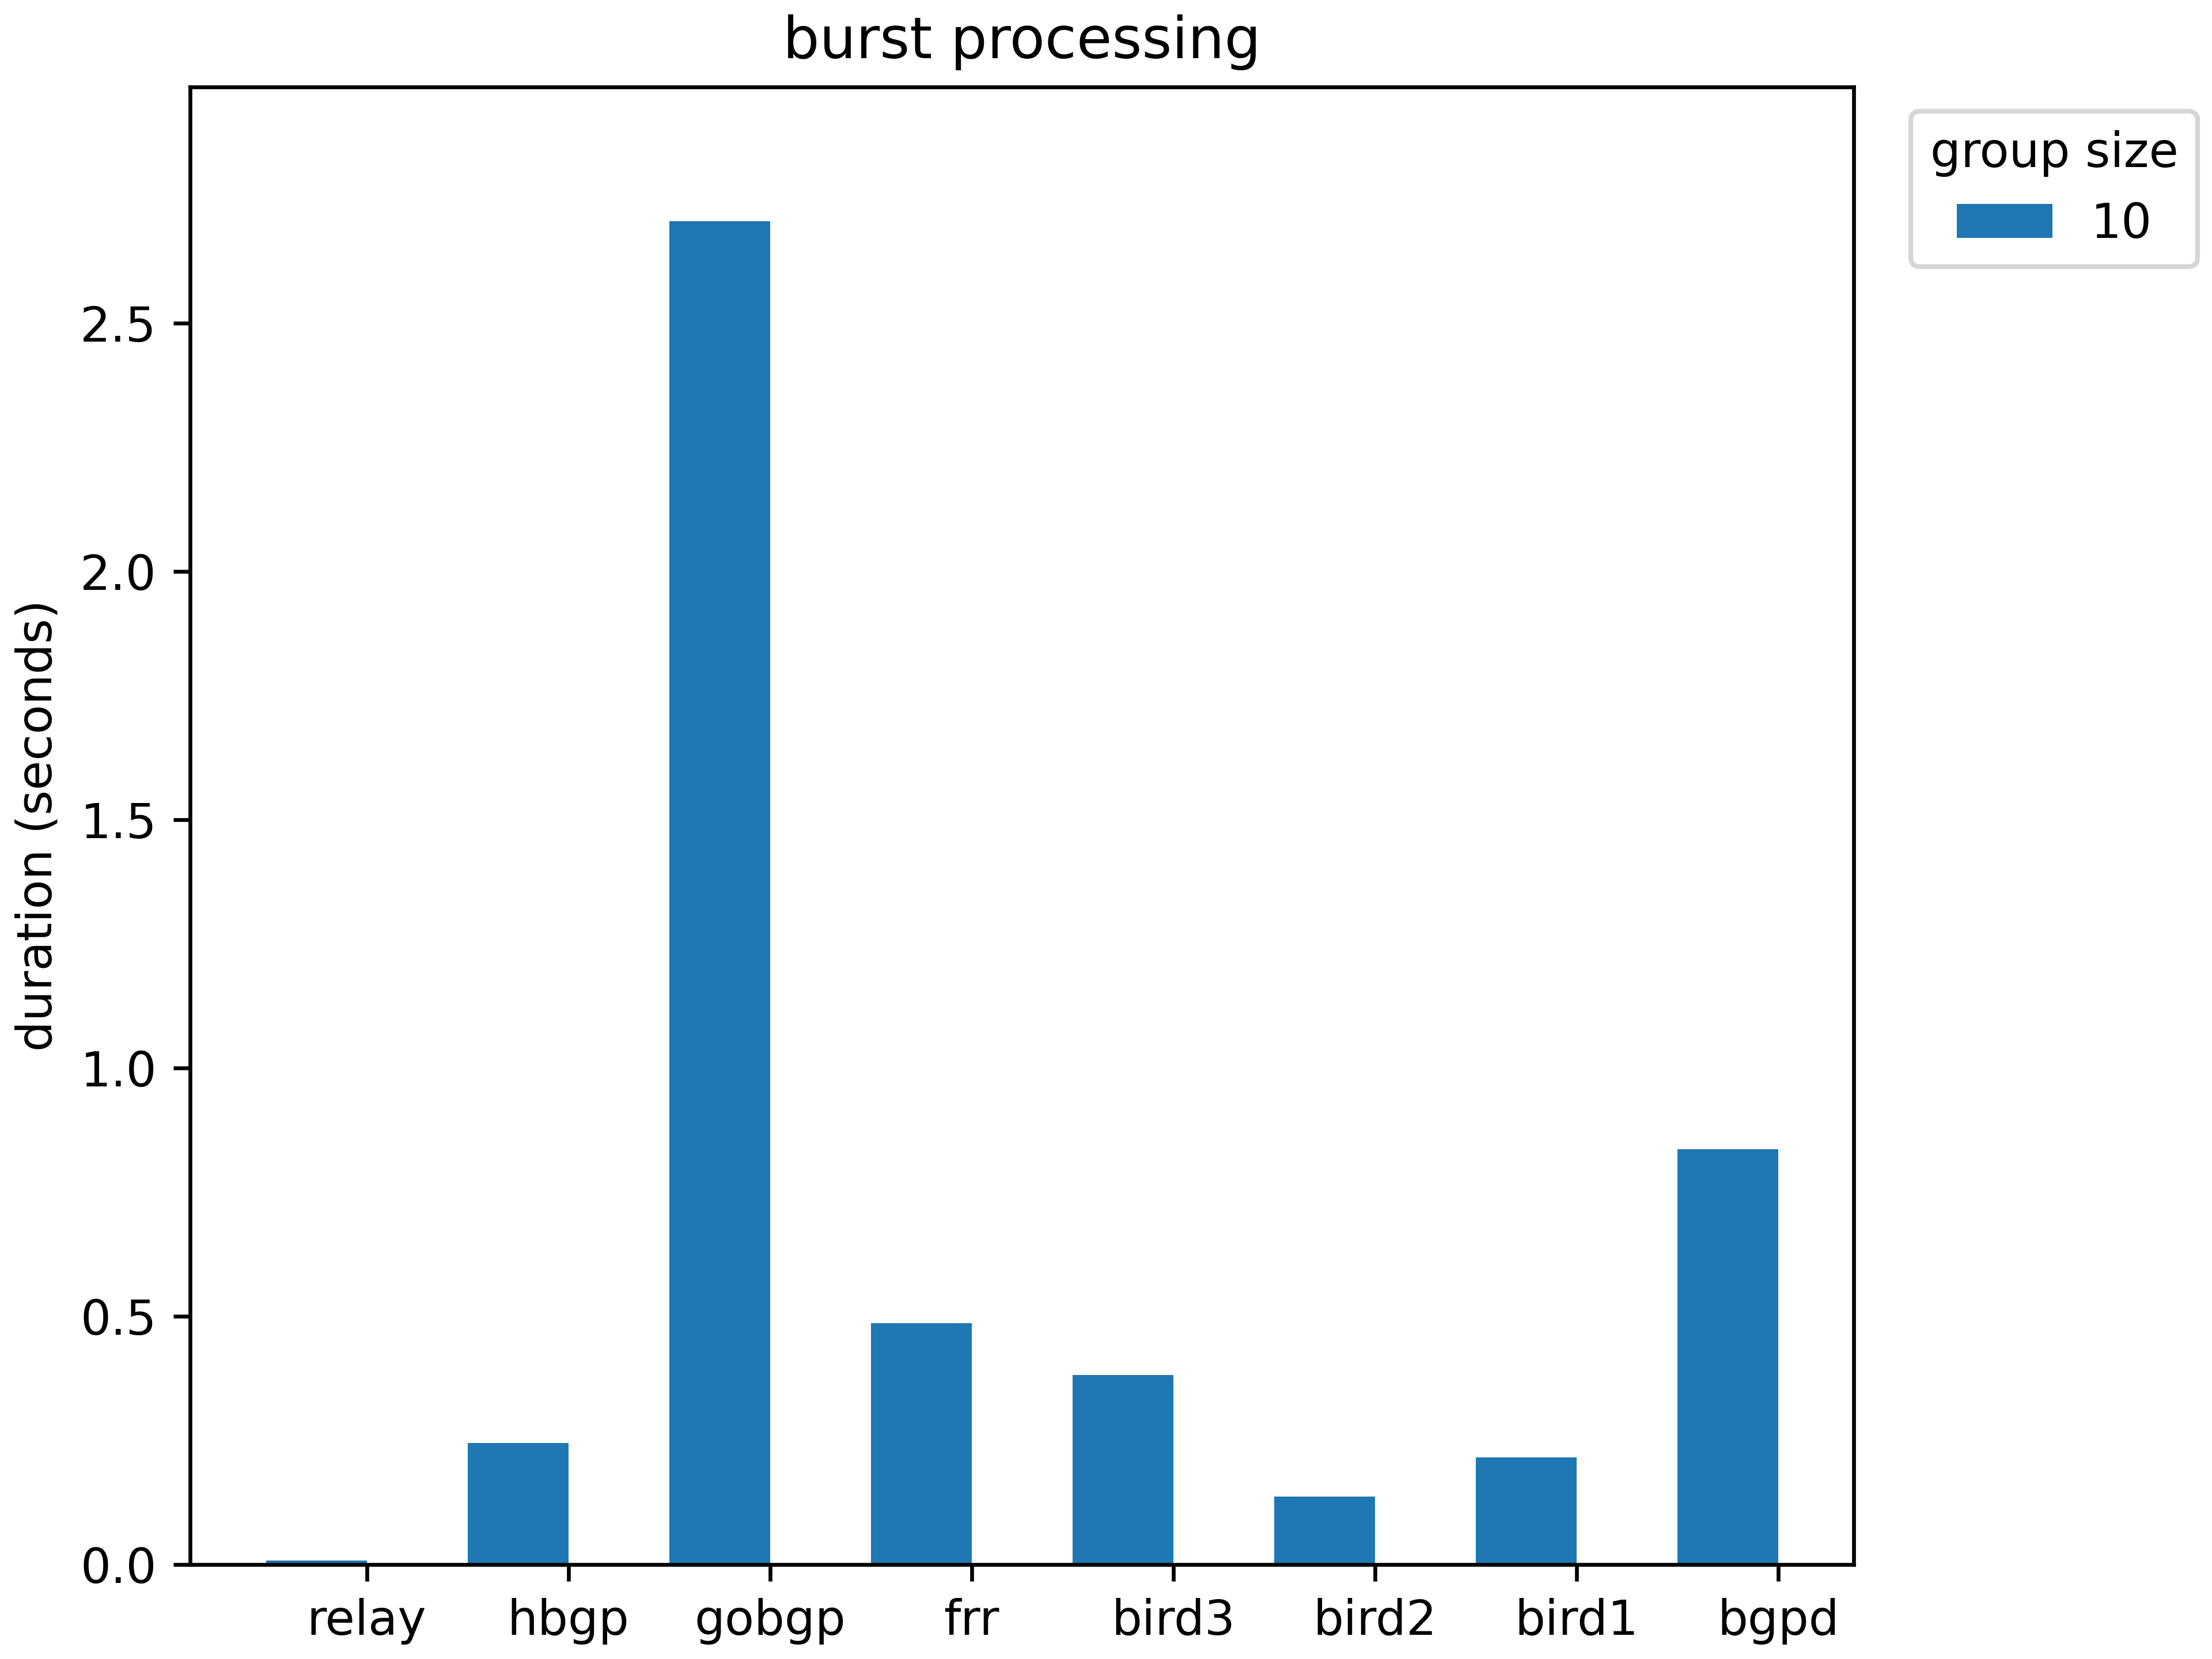
\includegraphics[width=0.7\linewidth]{1750178719.png}
    \caption{sample figure from report tool}
    \label{fig:1750178719}
\end{figure}

A more complete example is this one: \ref{fig:1750175110}.
for which the command was:
    \begin{lstlisting}
    ./report2.py mongo host=alef01 tag=samples3 targets=bird1,bird2,bird3,frr,hbgp,bgpd,gobgp save
    \end{lstlisting}

  \begin{figure}[H]
    \centering
    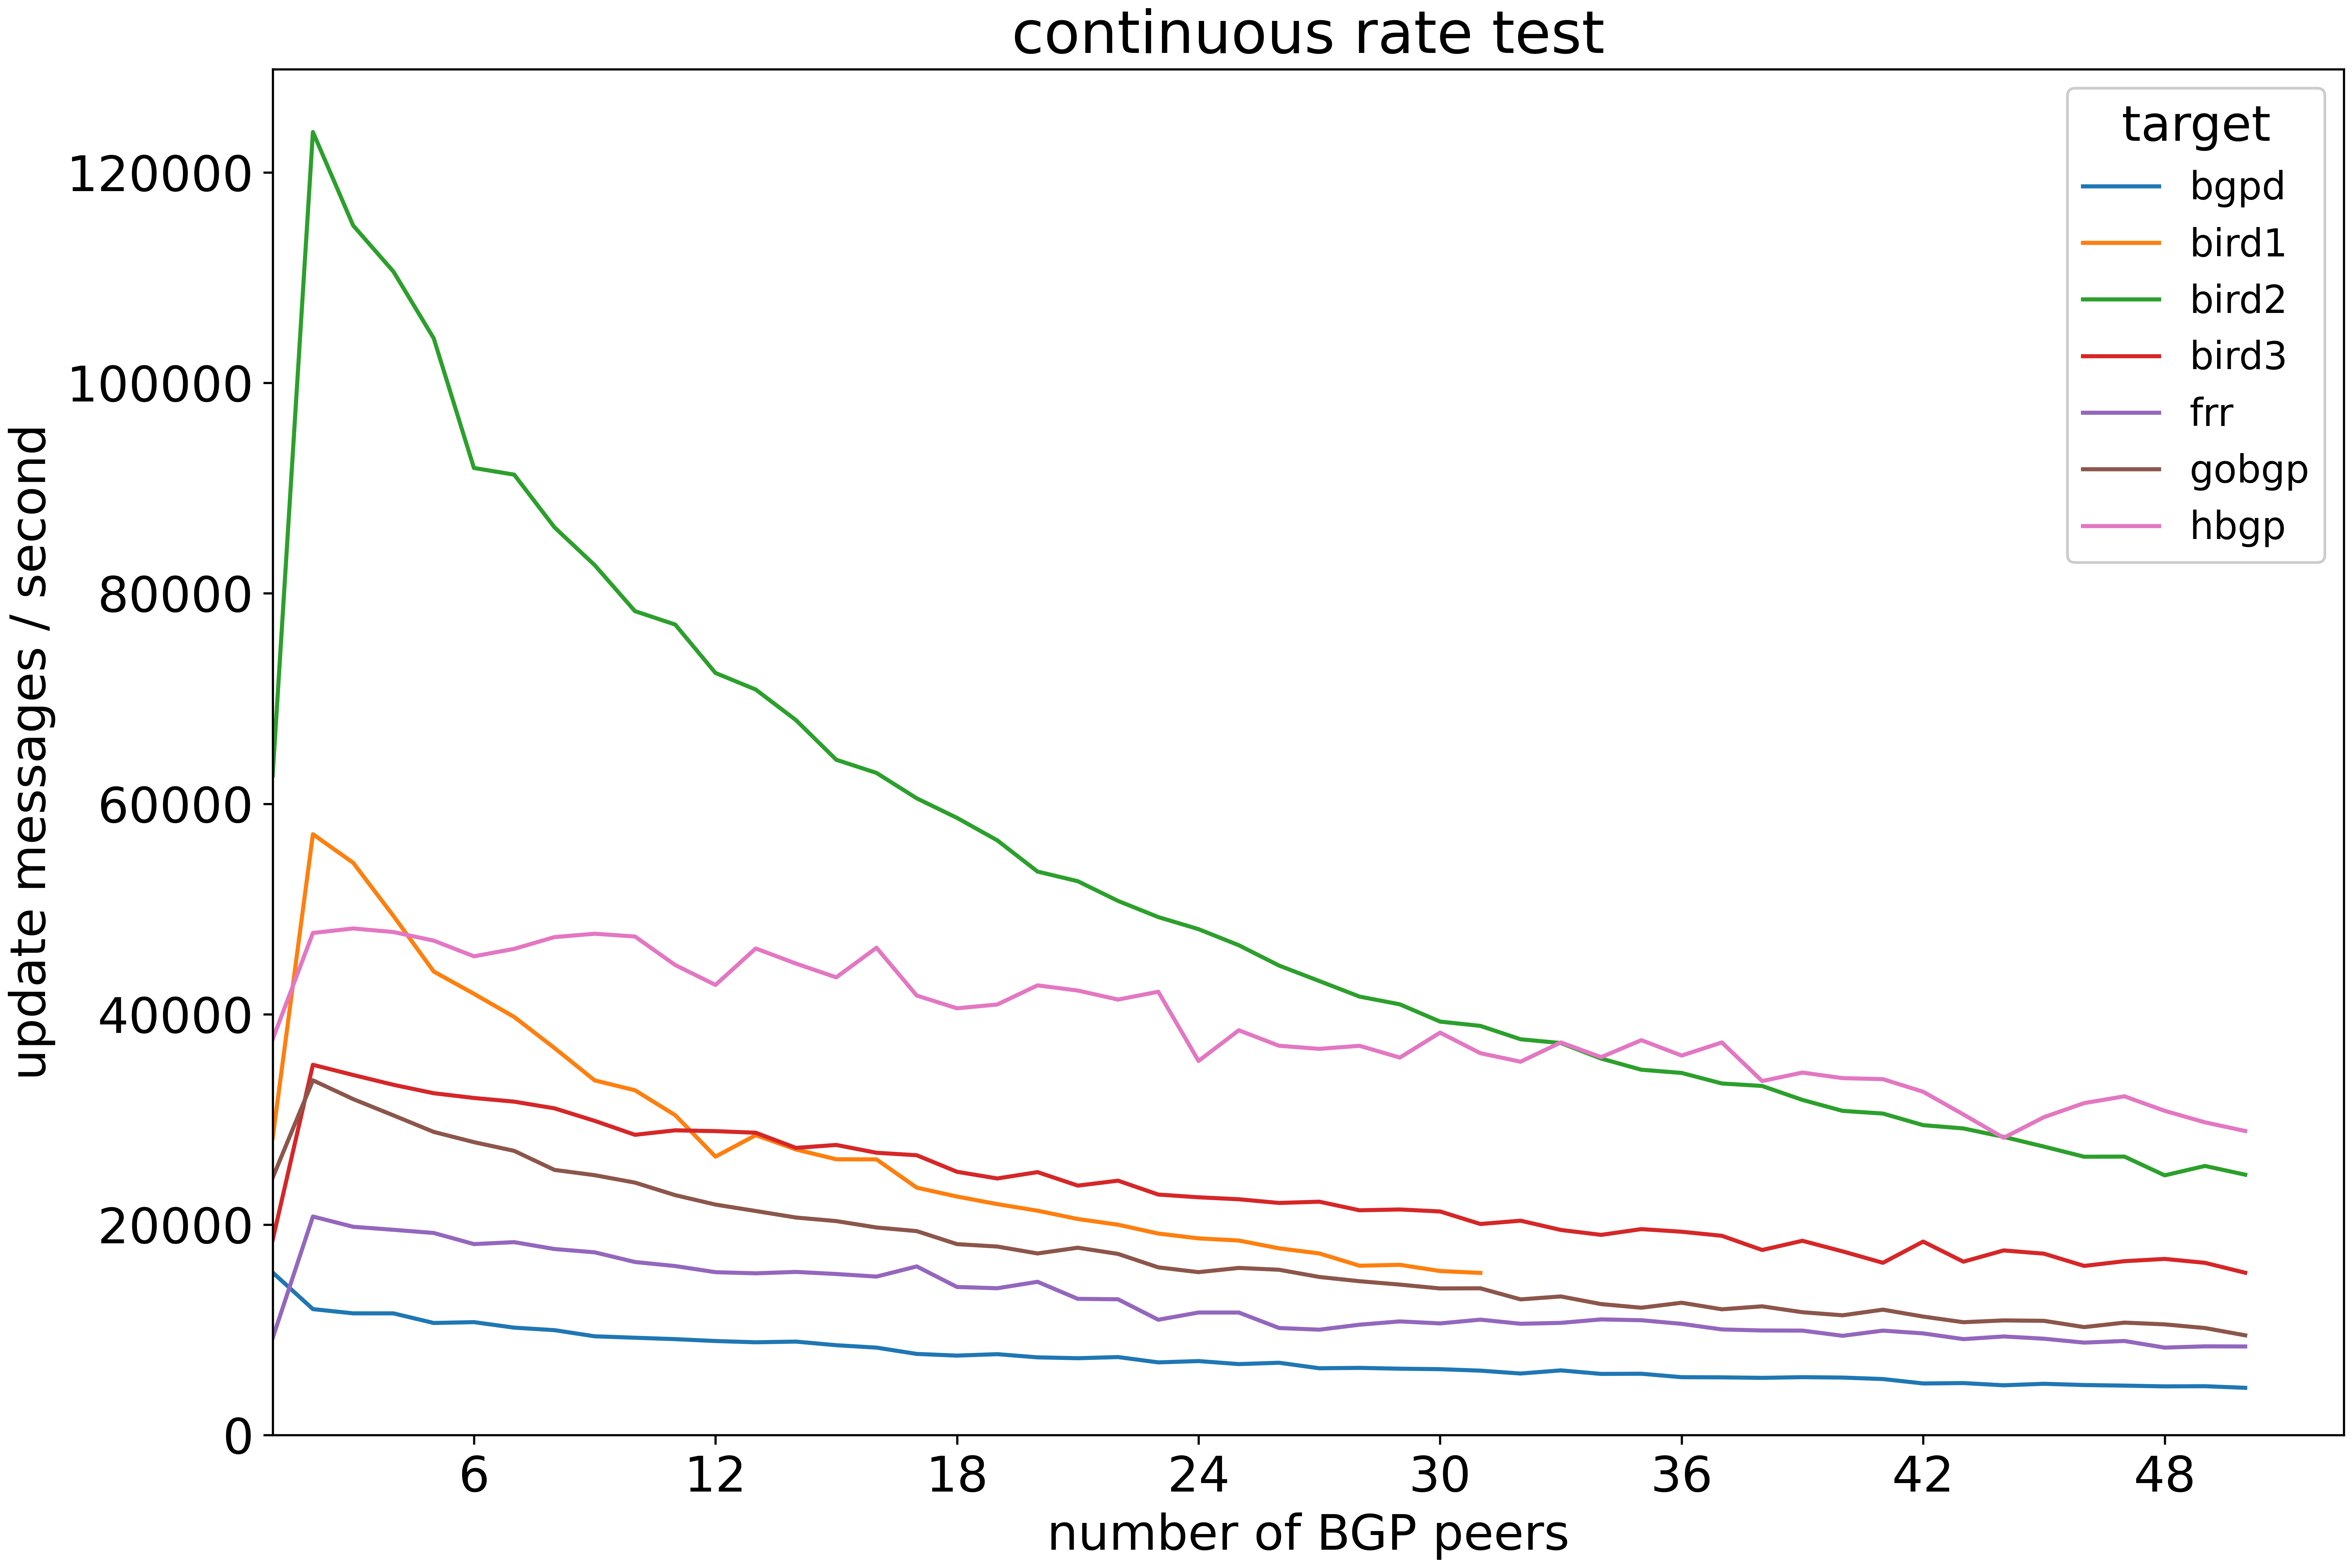
\includegraphics[width=0.7\linewidth]{1750175110.png}
    \caption{sample figure from report tool    }
    \label{fig:1750175110}
\end{figure}




\subsection{Baseline Performance: Single-Session Scenarios}
In order to establish a set of baseline measurement profiles, in this section we focus our performance analysis on the single session scenario using the metrics discussed in the previous section.
Our measurement results are presented in Table \NH{XXX?}, reporting the mean and the standard deviation of each measurement across 50 runs.
In order to demonstrate the low measurement overhead of our platform, the table reports additionally the performance measurements of our custom BGP relay implementation.
The relay BGP speaker completes the table transfer in less than 90msec, while the processing of the route updates complete in approx.
30 msec.
This measurements suggest that the impact of our measurement in the overall latency measurement is less than 10\%.
In parallel, our system generates 4x more updates than the BIRD2 speaker can process, the fastest BGP speaker in this measurement.
Furthermore, our measurement highlight that there is a significant latency difference between a table transfer and a route update for most speakers.
This can be attributed to the significant number of memory allocations that the speaker needs to perform in order to create the required state for each new route.
In terms of performance, we highlight that BIRD2 achieves the best performance across all metrics.
In addition, BIRD2 exhibits a non-negligible performance improvement in comparison to BIRD.
Specifically, BIRD2 processes 100 msec faster on average the table transfer and the route update and its average processing rate is improved by 15\%.
FRR is significantly slower than BIRD and BIRD2, especially for the average processing, which is 4x time slower in comparison to BIRD2.
Nonetheless, from a network manager perspective, FRR supports series of configuration options, not available in BIRD.
OpenBGPD performance is measured to be somewhere between the two systems.
Finally, GoBGP exhibits the worst performance in comparison to the rest of the BGP speakers.
During our measurements, we note that the GoBGP process was saturating 6 CPU cores, which suggests that the speaker was using effectively its multi-thread capabilities.
The measurement results suggest that the use of a high-level language (Go) can have an impact on the performance of a BGP speaker, due to features like automated garbage collection, while enabling multi-thread support in a BGP speaker is not guaranteed to improve overall performance.

% Original heading: \subsection{Multi-session performance}
\subsection{Scalability Analysis: Multi-Session Performance}
In order to perform this measurement, we use the ability of kakapo to establish multiple sessions towards a speaker and measure the average processing latency of a table transfer (Figure~\ref{fig:tbl-transfer-scalability}) and a 50k route update batch (Figure~\ref{fig:ssbt-scalability}) for a varying number of active BGP sessions.
Furthermore, we extend our rate estimation experiment and consider two new scenarios: the route updates are sent over a single session (Figure~\ref{fig:ssrt-scalability}) or the route updates are sent in parallel from all sessions (Figure~\ref{fig:msrt-scalability})~\footnote{In this measurement, we omit GoBGP from Figure~\ref{fig:tbl-transfer-scalability}, because the latency was extremely high and present results for up to 10 active sessions in all other figures, since the speaker kept resetting BGP session for higher session numbers}.

\begin{minipage}[c]{.49\linewidth}
	\centering
	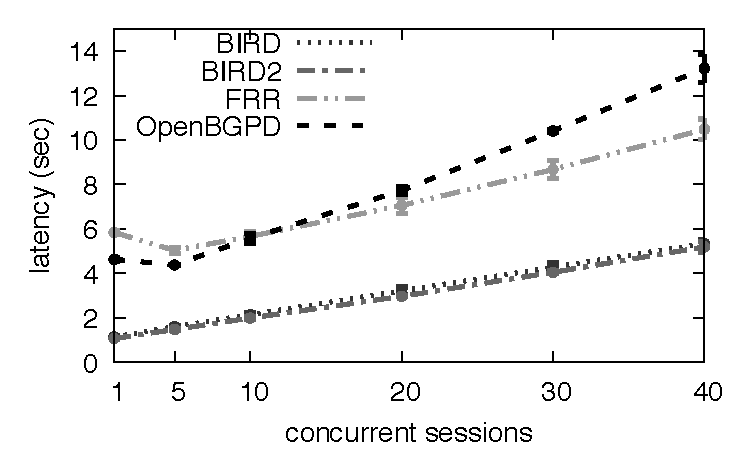
\includegraphics[width=\linewidth]{images/table-transfer-scalability.pdf}
	\captionof{figure}{Table transfer latency (800k).}\label{fig:tbl-transfer-scalability}
\end{minipage}
\begin{minipage}[c]{.49\linewidth}
	\centering
	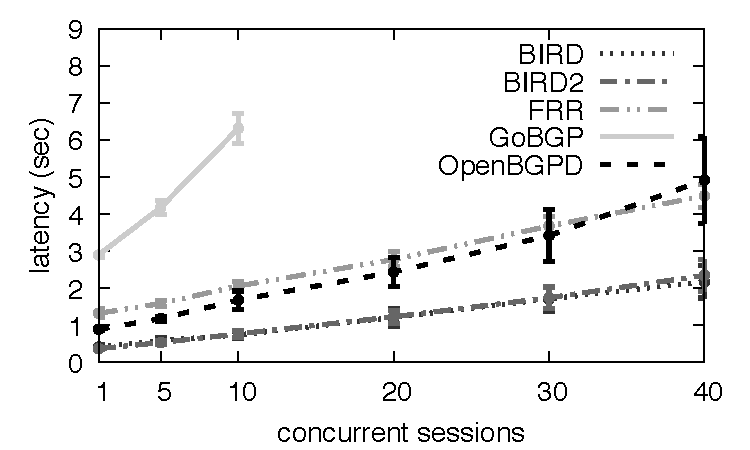
\includegraphics[width=\linewidth]{images/ssbt-scalability.pdf}
	\captionof{figure}{Route update latency (50k). } \label{fig:ssbt-scalability}
\end{minipage}
\hfill
\begin{minipage}[c]{.49\linewidth}
	\centering
	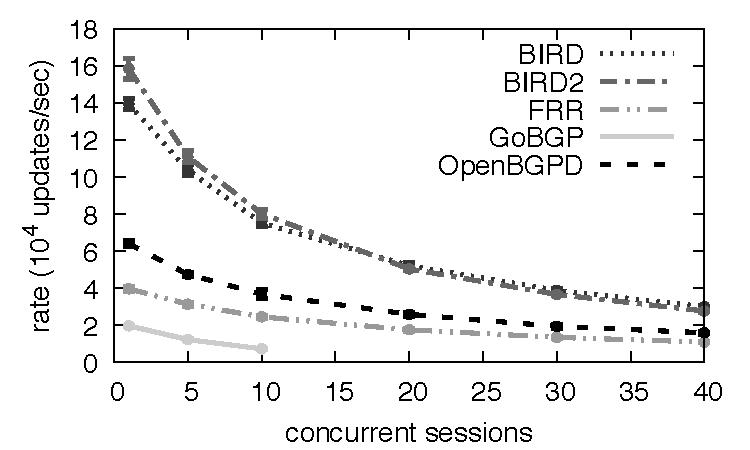
\includegraphics[width=\linewidth]{images/ssrt-scalability.pdf}
	\captionof{figure}{Single-session burst rate.}\label{fig:ssrt-scalability}
\end{minipage}
\begin{minipage}[c]{.49\linewidth}
	\centering
	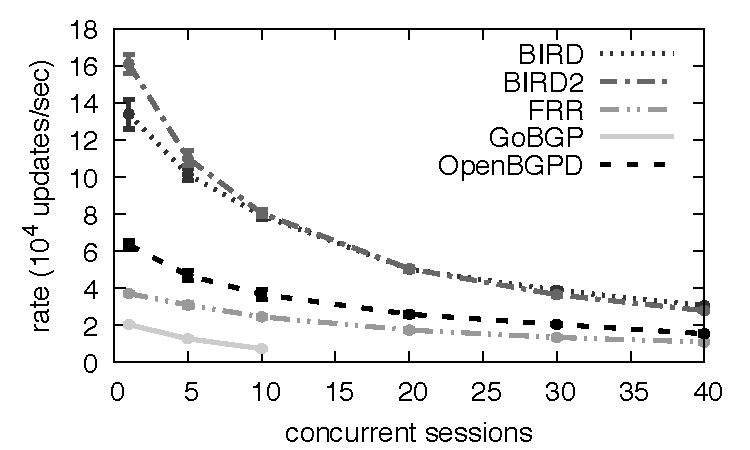
\includegraphics[width=\linewidth]{images/msrt-scalability.pdf}
	\captionof{figure}{Multi-session burst rate.} \label{fig:msrt-scalability}
\end{minipage}
\vspace{1em}

\paragraph{\textbf{Analysis}}
Firstly, we highlight that all speakers exhibit a very significant performance reduction as the number of active sessions increases.
This behaviour is consistent in table transfer, update burst and continuous rate measurement scenarios.
BIRD and BIRD2 appear to experience a significant processing rate reduction for high sessions numbers, since their processing rate halves as we increase the number of sessions from 1 to 10.
Nonetheless, this performance impact is not similar in the latency measurement, and both speakers exhibit a sublinear performance decrease.
OpenBGPD and FRR exhibit a sublinear decrease in their performance for both latency and rate measurements.
These characteristics might be explained either by the employed lookup structures, which increases its lookup times for large route counts, or the internal processing scheduling mechanism.
Secondly, for all BGP speakers, BGP performance varies only slightly when route updates are spread across multiple sessions.
Across all speakers, there a minor performance decrease on the order of 1\%-2\% on the average route processing rate.
This highlights that while all systems manage gracefully large update bursts coming from multiple parallel sessions, such as may occur during major route instabilities, however none of them manage to leverage the opportunity for parallelisation to actually improve performance.

\subsection{Impact of Transmit Window Size in Continuous Mode}
First we show as an example the results of a simple test case in which three different versions of the same open-source BGP speaker are deployed.
\ref{fig:rw_fig1}

\begin{figure}[H]
    \centering
    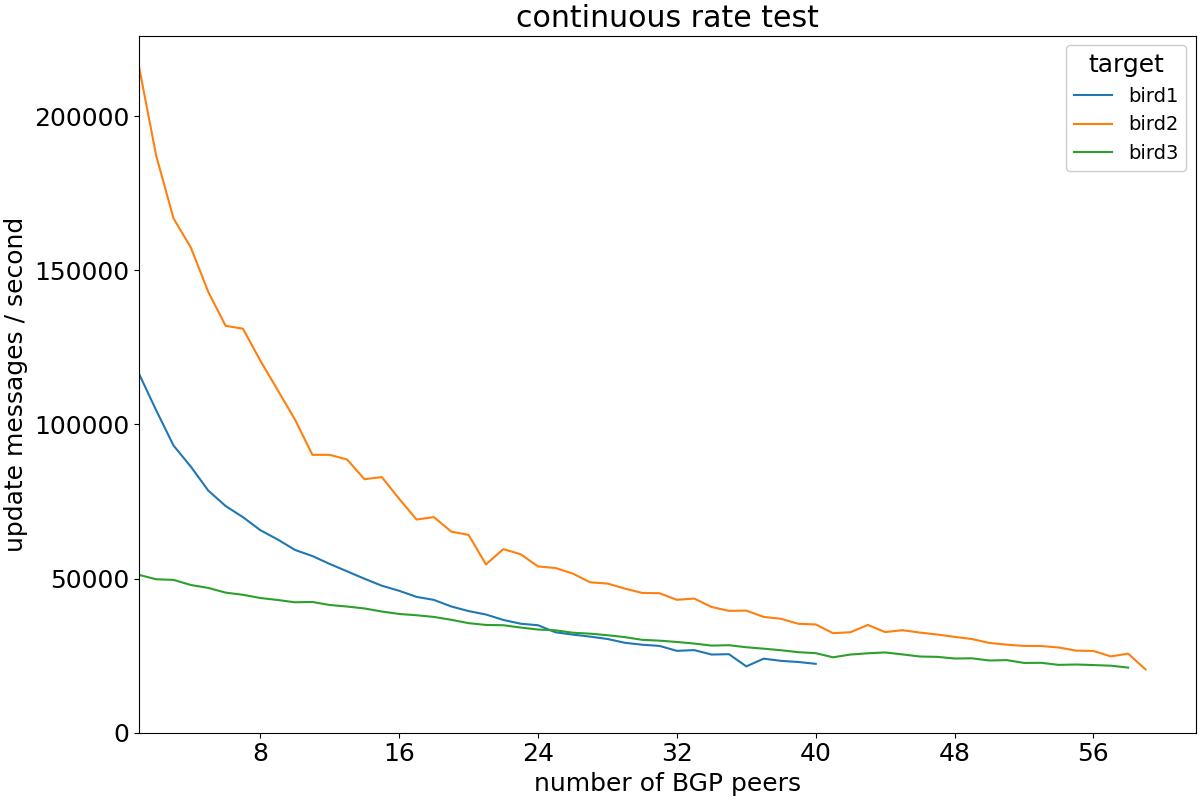
\includegraphics[width=0.7\linewidth]{ratewindow/Figure_1.png}
    \caption{rate test over varying number of source peers}
    \label{fig:rw_fig1}
\end{figure}

In the second version of the same graph the test results include the reference BGP implementation ‘relay’, which provides a benchmark measurement to give some confidence that even for the best performing BGP implementations, the measurement framework itself is not a significant drag on observed performance.
\ref{fig:rw_fig1a}

\begin{figure}[H]
    \centering
    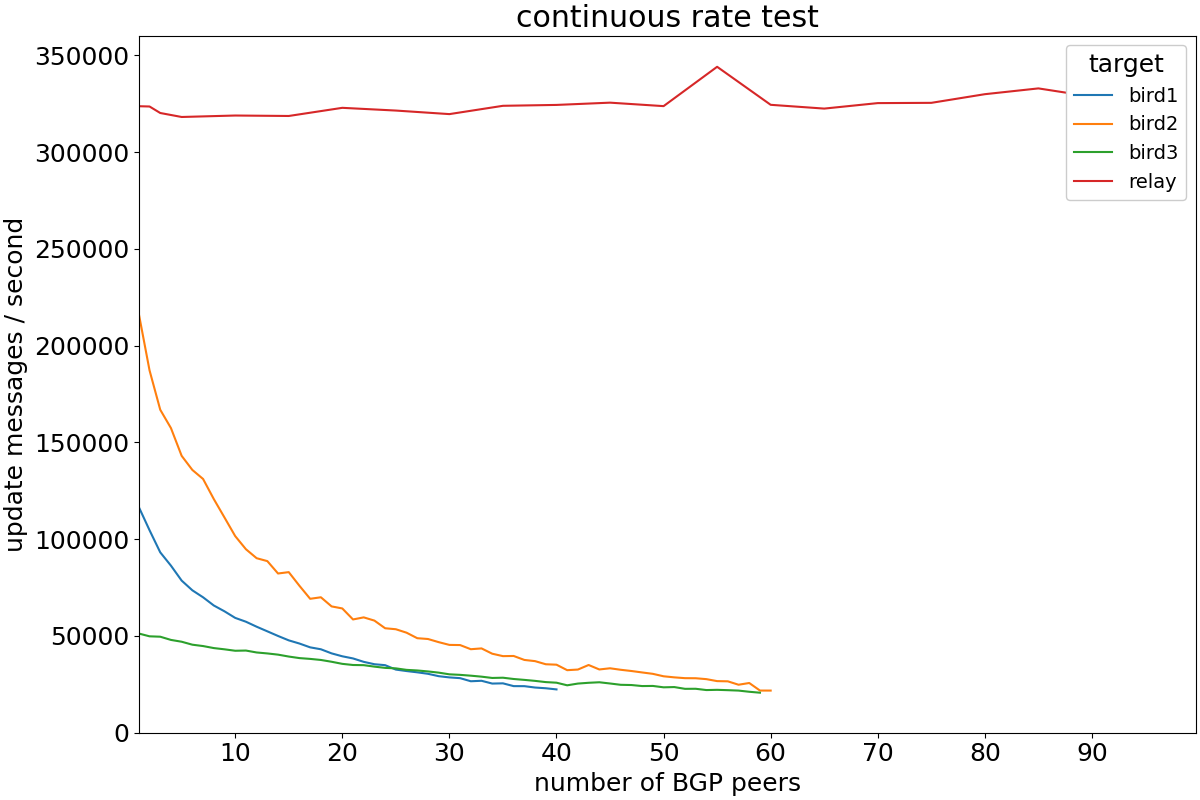
\includegraphics[width=0.7\linewidth]{ratewindow/Figure_1a.png}
    \caption{rate test over varying number of source peers - with `relay' baseline}
    \label{fig:rw_fig1a}
\end{figure}

In these next graphs, the impact of the chosen window size is evaluated.
We hypothesise that for any given BGP speaker there should be some optimal value of window size, a value which is relatively small compared to the full table size bursts applied in Kakapo block mode.
We can also expect that, for very small windows sizes, the lower rates achieved may ultimately be limited by processing latency in the BGP speaker, which can be seen as a distinct measure to `performance under sustained load', but is nonetheless an independent and meaningful performance metric.

\begin{figure}[H]
    \centering
    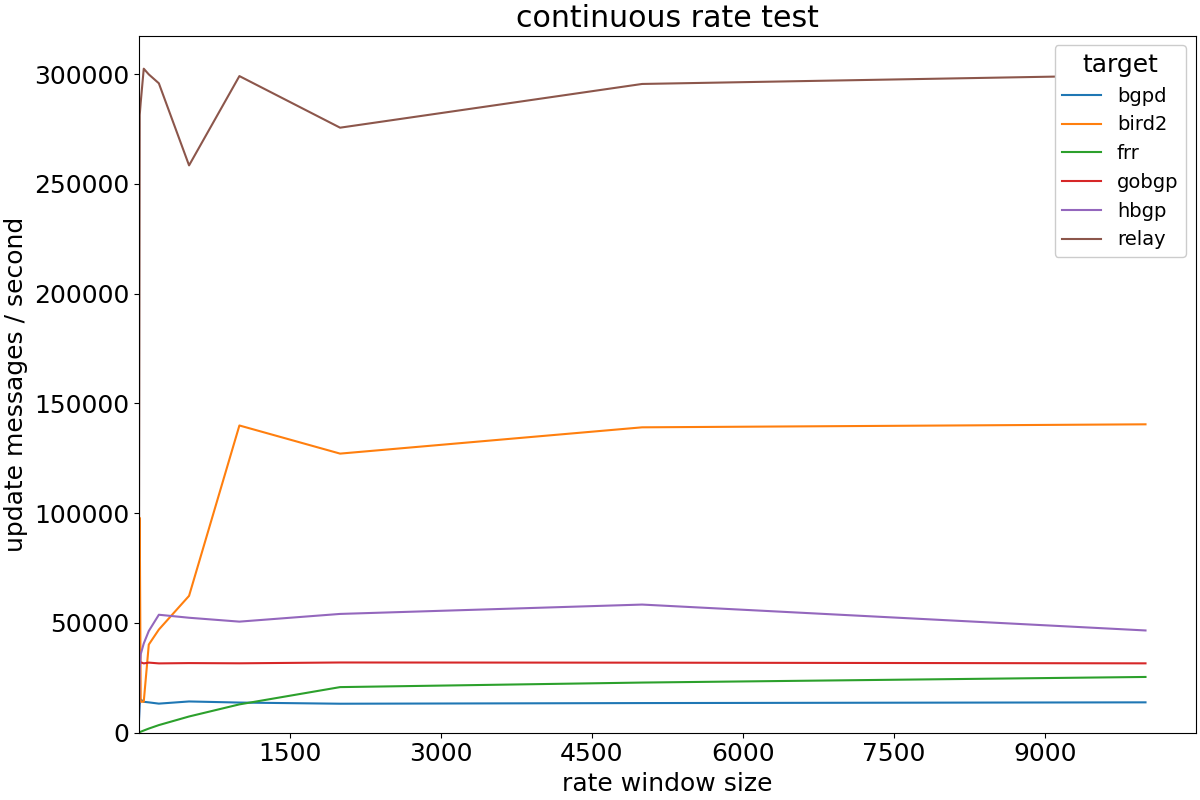
\includegraphics[width=0.7\linewidth]{ratewindow/Figure_3.png}
    \caption{rate test - fixed peer count, adjusting the rate transmit window }
    \label{fig:rw_fig3}
\end{figure}

\paragraph{analysis of \ref{fig:rw_fig3}}
Absent some interesting anomalies around the smaller window sizes it can be seen that above a transmit window size of 2000 messages, all BGP speakers approach some reasonable level of consistency for throughput.

There are some  anomalies, the most obvious and distinct is the behaviour of FRR \- for very small window sizes, FRR does much worse than any other BGP speaker.
This is quite easily explained by the observation that FRR is the only BGP implementation tested which universally applies the default Linux TCP DELAY (Nagle algorithm).
The newly implemented BGP endpoints all set the Linux socket option TCP\_NODELAY, and it is safe to assume that the others, apart from FRR, do the same.

Another anomaly arises in the case of bird2, better seen in this expanded version of the figure, limited to smaller windows sizes:

\begin{figure}[H]
    \centering
    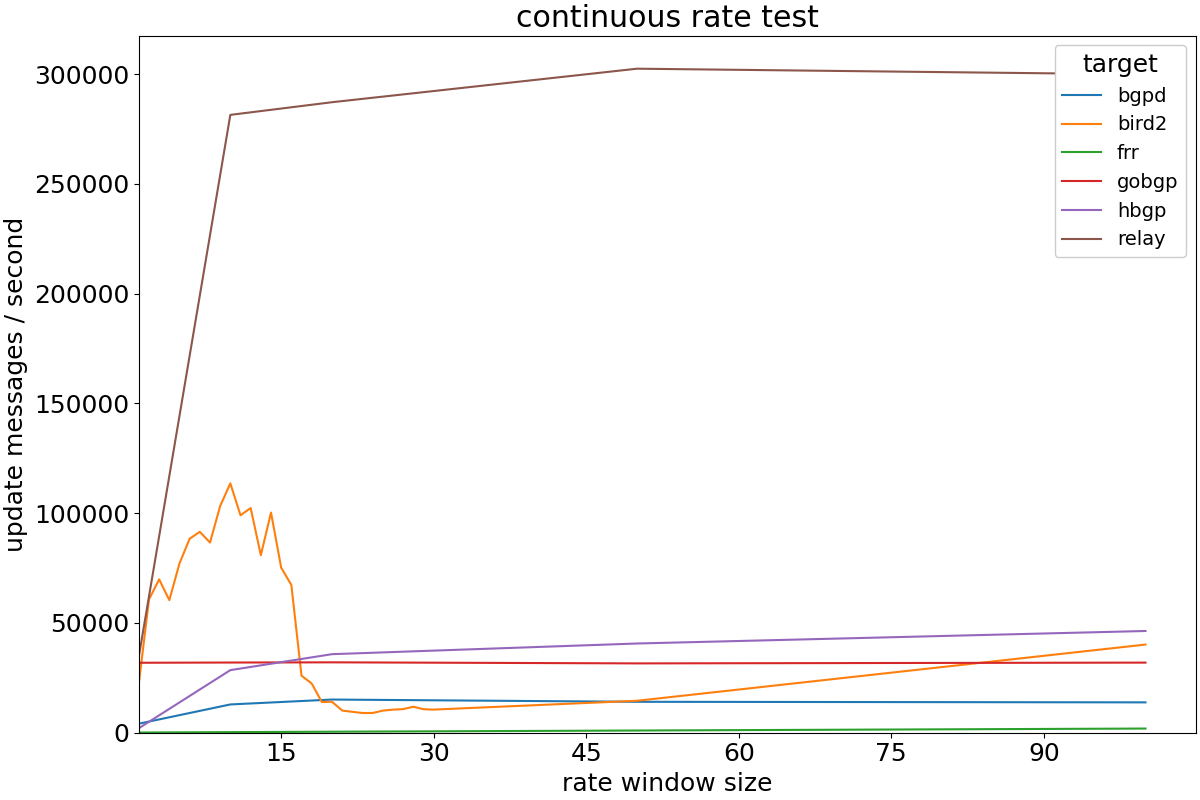
\includegraphics[width=0.7\linewidth]{ratewindow/Figure_3a.png}
    \caption{focus on bird2 sensitivity to small transmit window sizes }
    \label{fig:rw_fig3a}
\end{figure}

Here it can be seen that there is a real and repeatable anomaly in the case of bird2,for window sizes less than 20.
There is no obvious explanation for this effect.
This graph also illustrates significant differences between each of the other BGP speakers: since the performance in this realm is effectively a measure of latency, the measurements are not entirely trivial, and the merit ranking is strikingly different from others in this study:
\begin{itemize}
     \item For window sizes below 15, bird2 is ‘better’, followed by gobgp: gobgp is strikingly consistent, to such an extent that it could be worthy of investigation in its right.
     \item Then, in the realm of windows sizes from 15 to 100, consistent trends are established that extend up to the larger windows sizes of the main graph, the exceptions being FRR, for which a window size of 2,000 are greater is needed in order to achieve the best throughput of which it is capable, and bird2, whose actual and relative performance falls from best to 4th of 5\.
     \item At window sizes above 100 bird2 starts to reemerge as a much higher performer than the rest of the group, although it is still less capable than hbgp until the window size reaches 250.
     \item Bird2 reaches its best throughput of around 140k updates/sec at a window size of 1000; the next best BGP speaker, hbgp, achieves around 50k updates/sec in this scenario.
\end{itemize}

Note however that this test runs only a single source update peer: when a larger number of source peers is configured, bird2 performance degrades and eventually is overtaken by hbgp.

\begin{figure}[H]
    \centering
    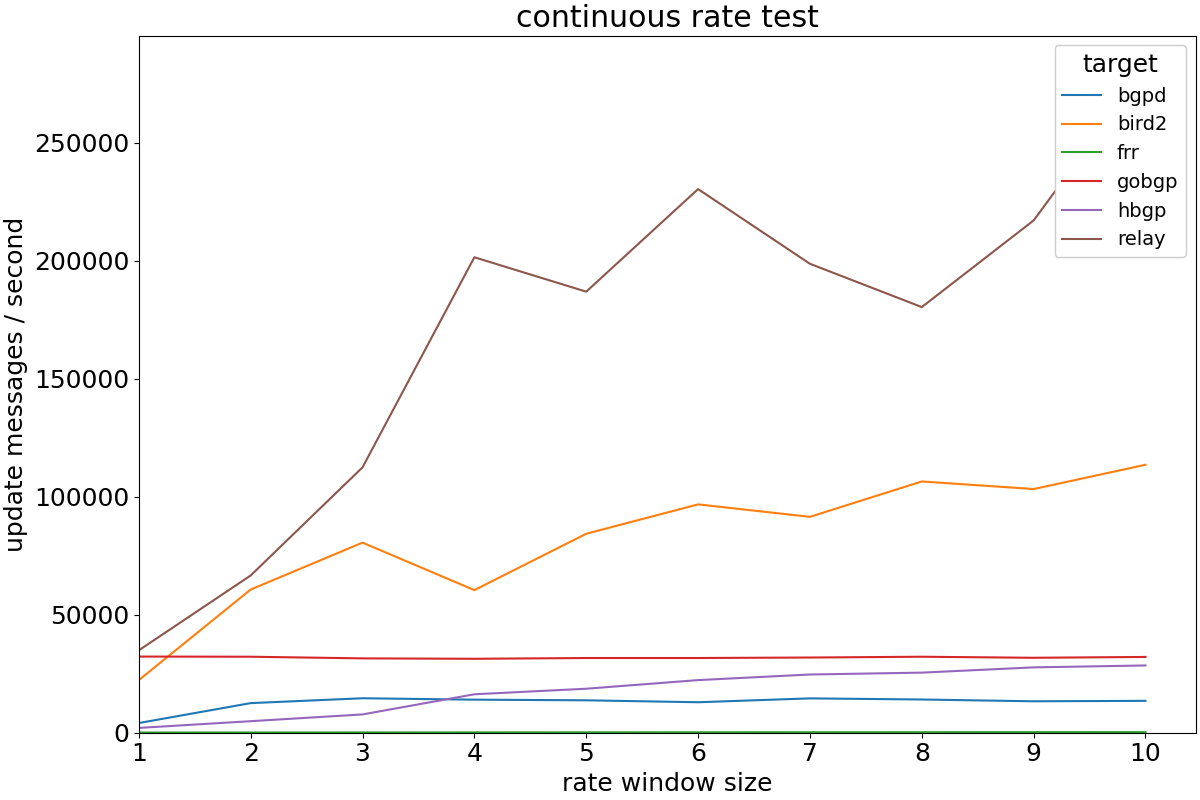
\includegraphics[width=0.7\linewidth]{ratewindow/Figure_3b.png}
    \caption{TBC }
    \label{fig:rw_fig3b}
\end{figure}

The final word should be said on the baseline measurements using the reference null bgp implementation, ‘relay’.
This greatly expanded view of the same rate data (\ref{fig:rw_fig3b}), achieved with the smallest, single digit, windows sizes, shows that until the window size reaches 4, the performance of bird2 is only slightly below the reference implementation, so that for this case it would be wise not to attach to much significance to the exact values reported.
However, since the gap between reference and bird2 widens and remains consistently wide for larger window sizes, it seems unlikely that the experiment ‘unfairly’ negatively represents the capability of bird2.
For higher confidence  insight,  the best technique would be to analyse packet trace data with accurate timestamps, in order to measure latency directly.
Since latency performance is not a major focus of the work, the refinement of the kakapo tool for precision latency measurement is left for future work.
This figure also serves to further underline the remarkable consistency of the metric for the gobgp case.

\subsection{Impact of Prefix Packing on Processing Performance}
The BGP message protocol supports a convenient and universally applied optimisation, which is to allow routes with common path-attributes to be advertised in a single Update message.
Other than as an optimisation, there is no semantic distinction between a single Update carrying \textit{N} routes, and \textit{N} Update messages, each carrying a single route, if the path-attributes otherwise remain identical.
Here, the practice of combining routes in this way is referred to as prefix packing.
The subject of investigation is how the usage, or otherwise, of `prefix packing' affect the performance of BGP speakers.
It is a worthwhile question, not least because the requirement to maintain packing structures on BGP Update flows presents a very serious challenge for designers of BGP systems, and especially for designs intent on parallelising processing as far as possible.
Were an otherwise `credible' new BGP system to be proposed, but one which often or always did not optimally pack routes in Update messages, it might be hard to gain acceptance for real-world applications.

\subsubsection*{Experimental Approach}
In these investigations the existing Kakapo measurement tool is deployed, applying a procedural variation to force all transmitted messages to be `unpacked'.
Kakapo supports this behaviour with a parameter `NOPACK', which is either globally enabled, or not (the default).
The measurement set reported is a repetition of the canonical, single peer, continuous, rate test, already described.
All of the standard BGP implementations are evaluated under NOPACK operation, as is hBGP \footnote{the baseline test tool relay is not reported - there exists some defect in the tool which prevents reliable completion of test runs.
It is the only known deficiency in relay, to-date.}

\subsubsection*{Experimental Results}
The table \ref{tab:packing} shows summary results, for sustained processing rate, and also for initial route table load (`conditioning').
With a single remarkable exception, all tested BGP speakers exhibit some degree of impact of unpacked operation.

\begin{table}[htbp]
\centering
`
\begin{tabular}{ccccc}
\toprule
\thead{BGP Speaker} & \thead{Rate \\ Packed Updates} & \thead{Rate \\ Unpacked Updates} & \thead{Percentage \\ Reduction} & \thead{ Reduction \\  Ratio} \\ \midrule
bgpd  & 13266          & 57683            & 435\%             &      
            \\
bird1 & 61384          & 45062            & 73\%              & 1.36            \\
bird2 & 131958         & 90549            & 69\%           
    & 1.46            \\
bird3 & 35521          & 29575            & 83\%              & 1.20            \\
frr   & 21642          & 14503            & 67\%   
            & 1.49            \\
gobgp & 33201          & 5297             & 16\%              & 6.27            \\
hbgp  & 42910          & 13192        
     & 31\%              & 3.25            \\ \midrule
vMX	& 4833		& 4461		& 92\%		& 1.08          \\
`
vIOS		& 2053		& 565		& 28\%		& 3.63           \\ \bottomrule
\end{tabular}
\caption{Comparative performance (Update processing rate - routes per second ) of BGP Speakers, when Update Prefix packing is disabled on the input stream}
\label{tab:packing}
\end{table}

\subsubsection*{Analysis}
The mainstream BGPs, BIRDx and FRR, handle the unpacked input with reasonable grace, the same time `fixing up` the suboptimal format for downstream peers, as does Juniper vMX.
Given that the raw message rate is a factor of 10 greater, a performance decline of 10\% to 30\% is not unreasonable.
The outliers are the BGP newcomers - gobgp suffers the most - a factor of greater than x6, and \hbgp by more than x3 - even though neither of them are able to re-aggregate the resulting Update stream.
Interestingly, the Cisco virtual router also performs poorly - performance drops by more than a factor of 3.
However, Cisco and the Juniper vRouters do at least re-aggregate the Updates on re-announcement.
An additional observation can be made, which is whether the BGP speaker under test packs prefixes when re-announcing them.
This observation is carried out by taking sample packet traces and analysing with Wireshark \footnote{This sample based analysis does not prove that the identified behaviour is uniformly applied, but it seems reasonable to assume that a mid-stream analysis of several updates in sequence is representative.
However, caution is wise on the assumption of consistent behaviour: it is known that early versions of FRR were prone, under stress, to not packing Updates received as packed.}
The observed behaviour is that for bird and FRR only \footnote{and also the Cisco and Juniper vRouters}, Updates are consistently packed.
No other implementation packed Updates, when those received, were not themselves packed.
OpenBGP/bgpd is perhaps the most surprising case, for two reasons - which may be related: OpenBGP is the only BGP implementation which actually runs faster in unpacked mode, in the continuous mode test, and, of all of the `mature'  BGPs, it is the only one which does not actively repack arriving unpacked Updates.

\subsection{Influence of the Execution Environment}
In this next graph the impact of test context is shown \- the same set of measurements is taken using a laptop execution environment, varying the power control settings between ‘performance’ and ‘power saving’.

\begin{figure}[H]
    \centering
    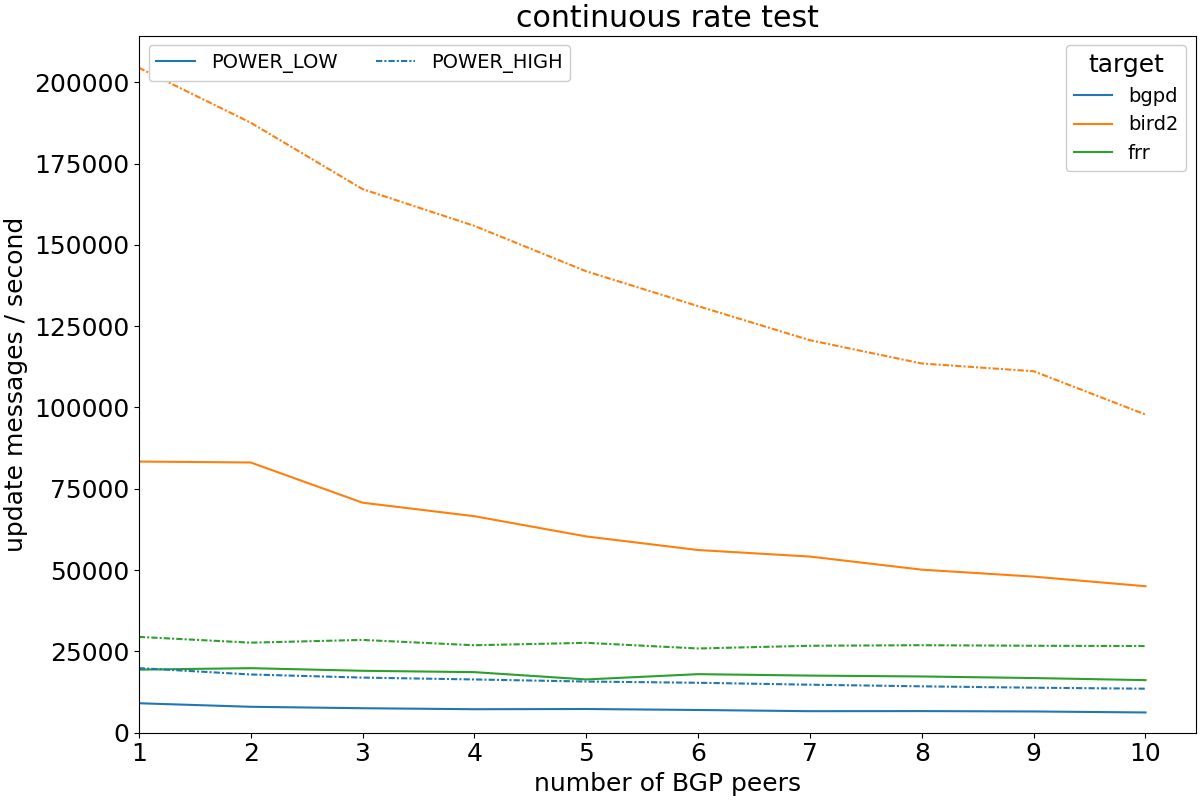
\includegraphics[width=0.7\linewidth]{ratewindow/Figure_2.png}
    \caption{TBC - fig 2}
    \label{fig:rw_fig2}
\end{figure}

Unsurprisingly, the performance changes, but it is noteworthy that the effect is not entirely linear.
For bird2, the low and high power performance ratio is between 2.2 and 2.5, whilst for frr the ratio is only between 1.5 and 1.6.
No examples are known where execution context changed actual relative ordering of targets, but it illustrates that careful curation of execution parameters is essential, and statements such as ‘BGP-x is 5x faster than BGP-y’ should be treated with great caution, even when the specific test and scale are made explicit.
The next graphs illustrate such pitfalls in more detail.
The first is the above graph, but with additional power contexts, of which one is running on another hardware platform \- a rack server with high memory and CPU count, while evidently less performance on a single CPU.

\begin{figure}[H]
    \centering
    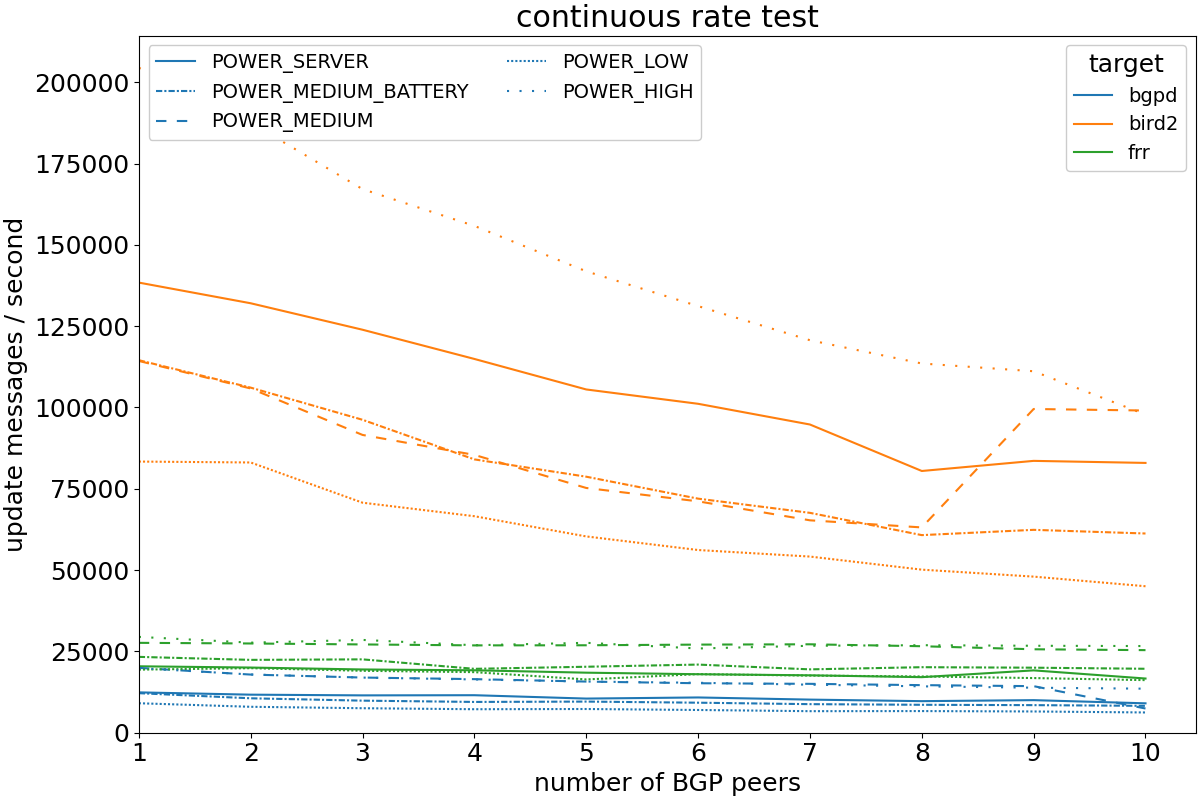
\includegraphics[width=0.7\linewidth]{ratewindow/Figure_2a.png}
    \caption{TBC - 2a}
    \label{fig:rw_fig2a}
\end{figure}

The especial factor here, other than that a laptop may often beat a high spec server when single or low core count applications are concerned, is that for the laptop, running on battery risks producing highly unreliable outcomes.
To safeguard against this source of inconsistency the kakapo framework records power supply status and when graphing experimental data records which show BATTERY as power source should be discarded.
And of course, for comparative purposes data from different hardware platforms should rarely be processed in the same analysis.
The above graph is the only case in which data from two hardware platforms has been combined for any reported experiments.
One more interesting observation selected from the same dataset:

\begin{figure}[H]
    \centering
    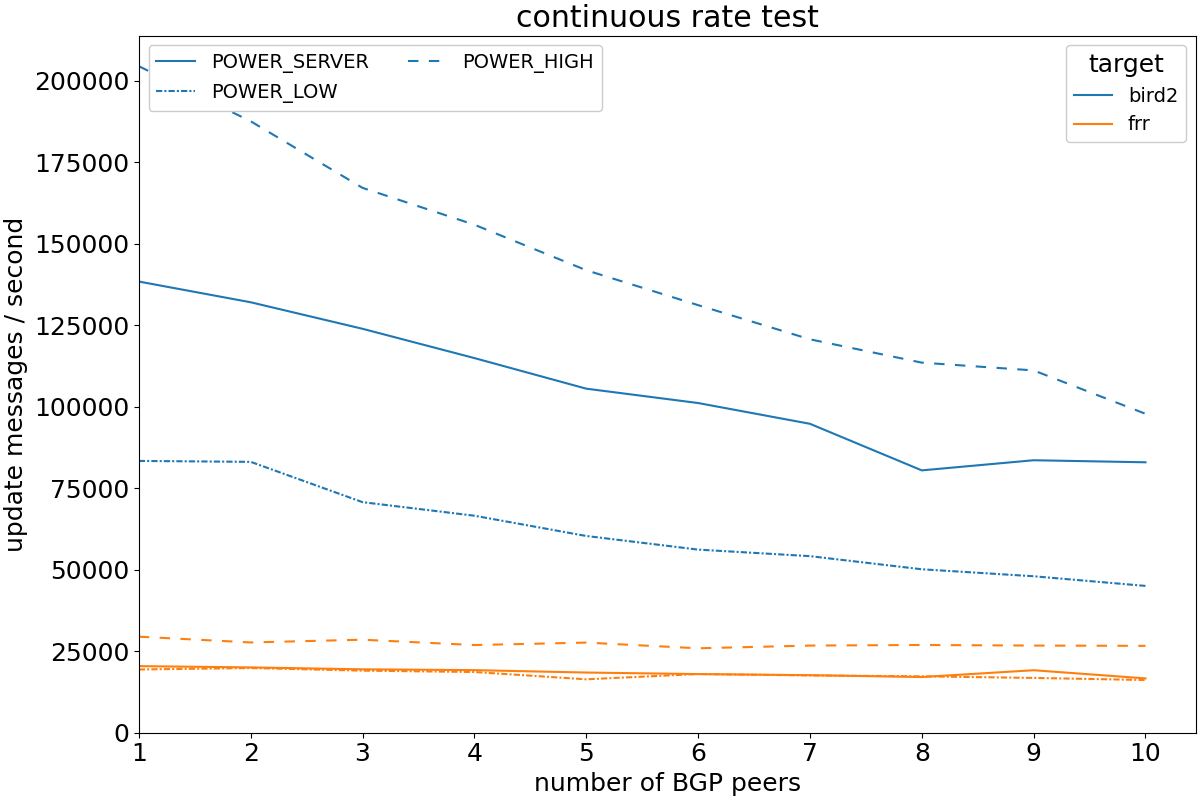
\includegraphics[width=0.7\linewidth]{ratewindow/Figure_2b.png}
    \caption{TBC - 2b}
    \label{fig:rw_fig2b}
\end{figure}

Here, the remarkable observation is that, for the frr workload, the laptop ‘power-saving’ performance is approximately the same as the server, yet for bird2 workload the server is as close to laptop ‘performance’ mode as to ‘power-saving’ mode.

\section{Conclusions}

kakapo has enabled the qualification of performance and stability of the new and novel BGP implementation, \hbgp.  In doing so, it has also provided significant insights into
\begin{myitemize}
    \item the challenges of evaluating BGP speaker performance
    \item the variability and performance envelope of well some known BGP implementations
    \item significant, and in some cases serious, shortcomings, at least as regards use for core IDR, in some of the platforms investigated.
    \item cautionary experience for those undertaking BGP performance evaluations, based on simpler methodologies
\end{myitemize}

In particular, the development and application of the continuous mode testing capability shone surprising light on several BGP implementations, as did the work exploring larger number of concurrent peer sessions.

The discovery that the `gold standard' for BGP performance - bird2 - is not always as distinctive as initial work seems to show was interesting, as was the discovery that the latest version of bird - bird3 - is significantly slower than its sibling/ancestor, bird2.

The initial, and most important, aspect of the work with kakapo was to provide validation that the new BGP platform built for the wider project was, as far as can be measured, comparable and, in many cases, even faster than existing well known BGP implementations.
Whilst \textit{very} early versions of Haskell BGP were not as performant - in particular, the initial experiments using Software Transactional Memory (STM) \cite{GHC-STM} \cite{STM2005}.

However, the most important role of kakapo in the development of \hbgp was as a stress and soak-test tool, although even here, the experience of building and improving performance for BGP in Haskell was surprisingly painless; probably the more testing procedures were functional tests, which required interoperability with the range of BGP speakers available, and in various roles and topologies.

\bigskip

Perhaps the most important validations of all are  

\begin{enumerate}
    \item The viability and practicality of  Haskell  \hbgp, in its controller variant form, for use at IDR scale - showing that it is possible to introduce external programmability to a `normal' BGP speaker, albeit one written in Haskell, without significant impact on its ability to perform, at scale, and at speed.
    \item The viability of applying a very high level Functional Programming language in a new and highly challenging domain - it is can be asserted that it is possible to build safer, more reliable and more flexible network protocol systems than could ever be achievable in `C', given the well known limitations of the `C' language, and the current trend to replace `C' in mission critical applications, with safer alternates.  The proven productivity gains of using Haskell only serve to reinforce the point, that future network systems can, and surely will, no longer be written in `C'.
\end{enumerate}